\documentclass[12pt]{report}
\usepackage{suthesis-2e}
\usepackage{graphicx} %demo arg - doesn't load figs; makes rendering faster
\usepackage{apacite}
\usepackage{url}
\usepackage{booktabs}
\usepackage{pslatex}
\usepackage{setspace}
\usepackage{array,multirow}
\usepackage{tabularx} 
\doublespacing
\dept{Psychology}

\begin{document}
\title{Conceptual complexity and the evolution of the lexicon}
\author{Molly L. Lewis}
\principaladviser{Michael C. Frank}
\firstreader{Ellen M. Markman}
\secondreader{Noah Goodman}
\thirdreader{Thomas Icard} 
\fourthreader{Hyowon Gweon} 
 
\beforepreface 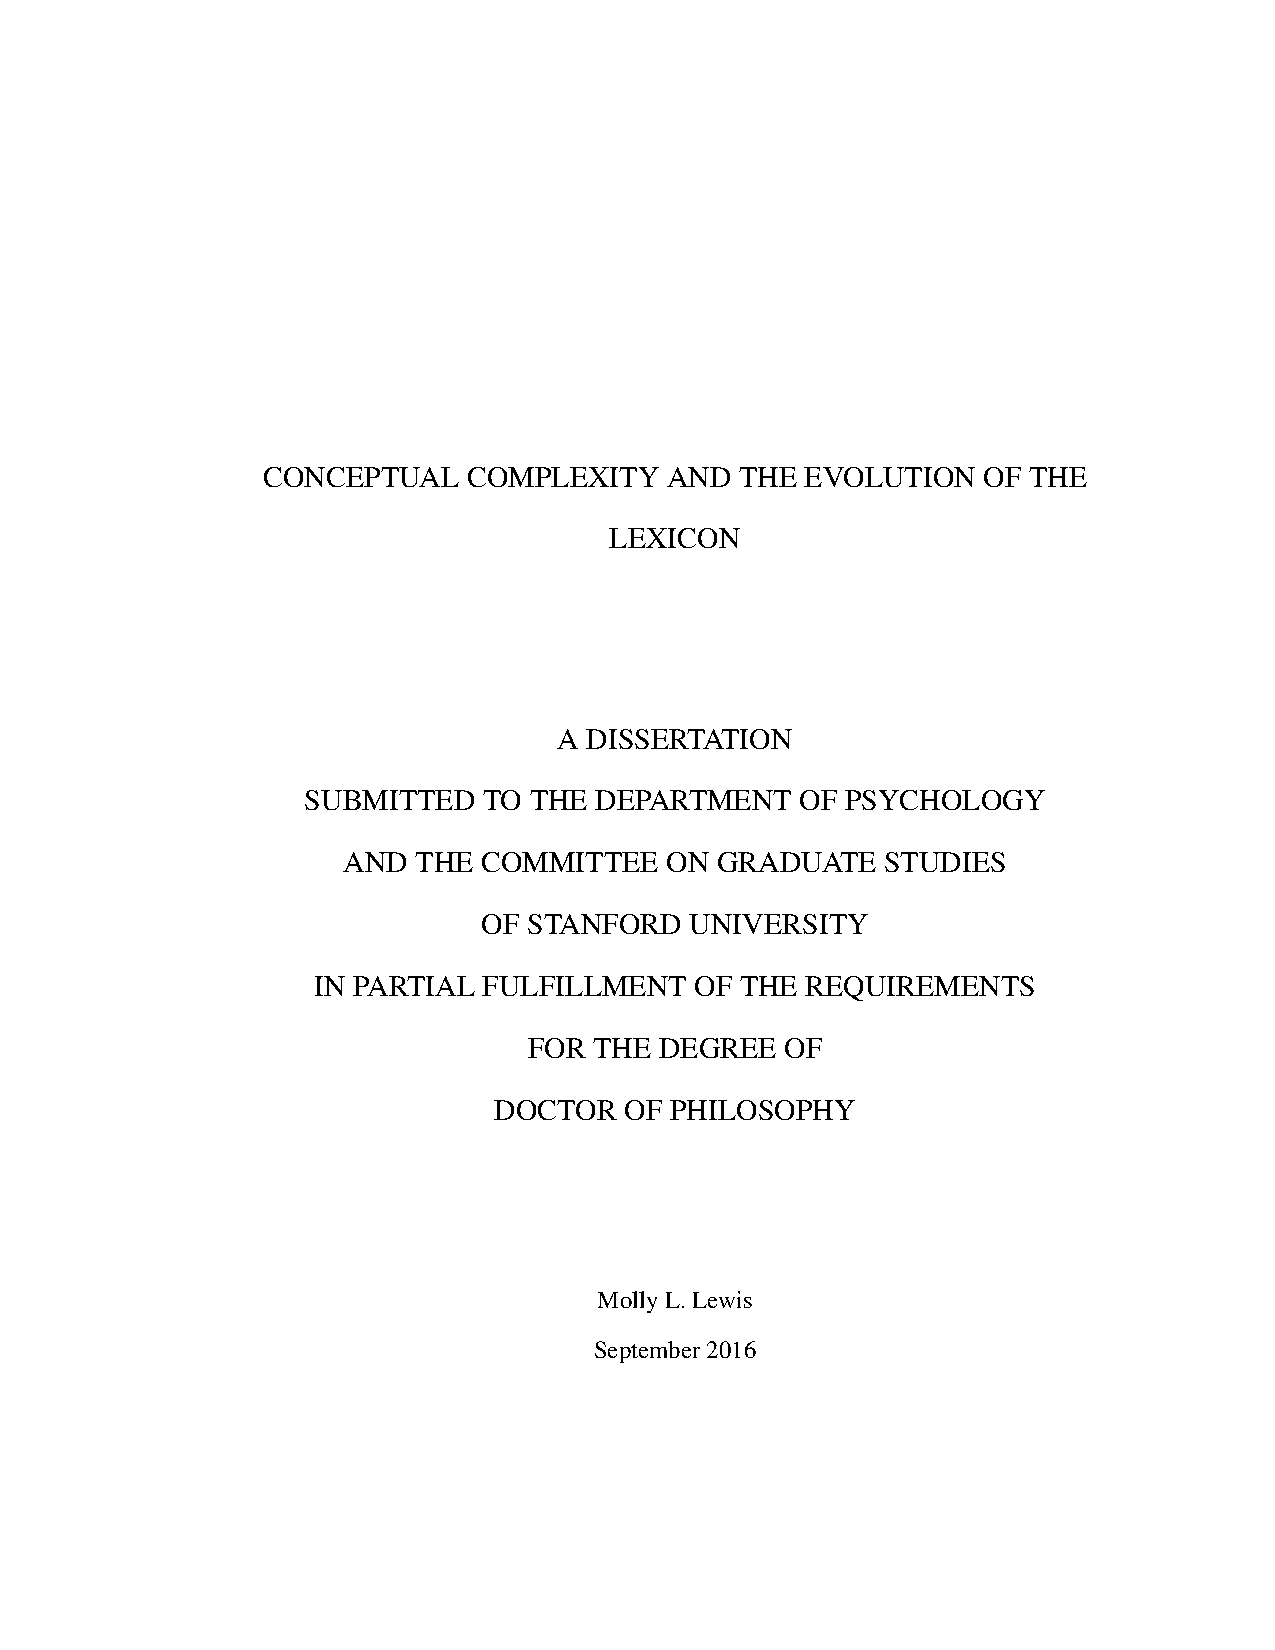
\includegraphics[]{disssertation.pdf}

\prefacesection{Abstract}
Natural languages are ripe with regularities. Where do these regularities come from? A parsimonious explanation is that these regularities emerge as a consequence of pressures within the broader context in which language is used: Communication among many cognitive systems. In this dissertation, I consider one particular regularity as a case study in how the dynamics of language use might shape language structure. Specifically, I focus on a bias in natural language to map long words on to conceptually complex meanings and short words on to conceptually simple meanings, or a {\it complexity bias}. Across a series of experimental and corpus studies, I explore whether languages and their speakers have a complexity bias, what conceptual complexity is, and what pressures might have lead to this bias over the course of language evolution. In the final chapter, I consider a broader range of linguistic phenomenon and examine how aspects of language use might influence these structures. 

\prefacesection{Acknowledgments}
I feel incredibly grateful to have had the opportunity and support to study a question that I find so fascinating for five years. On a short timescale, I thank the day-to-day cheer and camaraderie of the developmental community, my labmates, and my friends Kyla and Caitlin. On a longer timescale, I thank my advisor, Mike, for his intellectual guidance, but also his patience and kindness. On an even longer timescale, I thank my parents, Bonnie and Marshall, for their unconditional support of me and my pursuits. Finally, gratitude to my partner, Dan, for love and encouragement in an innumerable number of ways. This dissertation, I can say with certainty, is the product of (supportive) pressures at all of these timescales.  


%\setcounter{tocdepth}{1} TOC depth
%\FloatBarrier  % barrier to float placement of figures
%\caption[This appears in the list of figures]{This appears under the figure.} % caption in TOC vs under pic

\afterpreface

% https://github.com/samfcmc/ist-dissertation-latex-template - to make modular.
% OUTLINE: https://docs.google.com/document/d/1yaEI3AYkT3LTNtRKNAWOPFA0j6a3rUEjPA5yi8CWFGE/edit

%!TEX root = ../dissertation.tex

\chapter{Introduction}
\label{chapter:introduction}
%Chapter 1
%arbitrariness
%principles of comunication -> influence structure?
%timescales
%pragmatic equilibra in the lexicon
%accounts of the length of linguistic elements

%What is the relationship between processes at shorter timescales and language structure?

``Room for cream?'' asked the barista. ``Mm, yes -- just a bit" replied the customer. Mundane linguistic interactions such as this are the building blocks of daily experience. They are individuals making sounds to each other in an effort to coordinate their behavior in the physical world \cite{clark2006social}. These interactions are messy, variable, and highly unconstrained. Indeed it is this variability that gives language its vast expressive power \cite{hockett1960}. Yet, despite this appearance of irregularity, rich patterns in linguistic usage are revealed when we aggregate across instances of language use both within and across languages. At the level of syntax, for example, there is a strong bias in English to put subjects before verbs and, across languages, this pattern is attested more often than would be expected by chance alone  \cite{dryer2005order}. These types of probabilistic regularities exist at every level of linguistic structure --- from phonology, to semantics, syntax, and discourse --- and researchers from a variety of disciplines have taken as their project the goal of characterizing these regularities.

In this dissertation, I contribute to this effort with a particular focus on understanding how processes that unfold in language use shape language structure. What counts as language use? acquistion and More specifically, I ask how constraints of the cognitive system and communicative nature of language may function to shape language structure via language use.  

The answer  posits an indirect causal link between language use and language structure: Language use over time leads to regularities in linguistic structure. I will outline this answer by relying on an analysis of language separated by five different timescales. To preview, the hypothesis is that linguistic structure reflects language use as a consequence of local dynamics between adjacent timescales. A {\it timescale} is a unit of time over which significant changes in state occur. For example, the timescale of dinner is about an hour, where the significant changes in state are walking to the restaurant, sitting down, ordering food, eating the meal, then dessert, etc. In contrast, the timescale of gaining weight occurs over weeks, where the significant changes in state correspond to appreciable weight changes. Critically, the length of the timescales is determined by the change of interest.  [see chapt 2 for more timescales]

\begin{figure}
\begin{center} 
\includegraphics[width=6in]{figs/timescales1}
\caption{The five linguistic timescales. Each timescale is nested within a slice of longer timescales. The claim is that the dynamics between adjacent timescales (e.g., pragmatic and discourse) lead to changes over time in longer timescales. The developmental timescale is characterized by a particular person from a particular generation, $p_A$, interacting with a series of people over the lifespan. Repeated interactions with the same person, $p_B$, characterize the discourse timescale.}
\end{center} 
\end{figure}

In the case of language,  there are five timescales over which significant changes occur (Fig. 4). The first is the {\it pragmatic timescale}. The pragmatic timescale corresponds to the processes described by Horn's principles, and addressed in detail in Part I. The {\it discourse timescale} is a slightly longer timescale. The discourse timescale corresponds to repeated interactions with the same person; a series of pragmatic interactions. The third is the {\it developmental timescale}. The developmental timescale corresponds to the lifetime of an individual. It is composed of many interactions (on the pragmatic timescale), some of which with the same people (on the discourse timescale).  Many people interacting over their lifetimes lead to change at the {\it cultural timescale}. This is the timescale over which significant changes in language structure  occur (sometimes referred to as the ``language change" timescale). Finally, at the longest timescale, is the {\it evolution timescale}. All of the dynamics at lower timescales occur within a small slice in evolutionary time. While I will not have much to say about this timescale, its main significance is to situate the present claims with respect to claims about the innateness of language. Following \citeA{christiansen2008}, the suggestion is that there are aspects of language that are innate and constrain the dynamics of shorter timescales. Importantly, however, there are also  dynamics that take place at  shorter timescales, and these dynamics are the focus of the present section.

The phenomenon to be explained is why dynamics at the pragmatic timescale are reflected in structure at the cultural timescale. The proposal is that there are dynamics between adjacent timescales, and that, over time, these dynamics lead to change on longer timescales. Importantly, the character and phenomena of the dynamics between each pair of timescales are different. For example,  the dynamics between discourse and developmental timescales are reflected in cognitive changes in the mind of a particular speaker. In contrast, the dynamics between cultural and evolutionary timescales are reflected in genetic changes in linguistic abilities.

It is worth reflecting on the historical relationship between these two aspects of language. Across many schools of linguistics, theorists have made a theoretical cut between language use and language structure: {\it parole} vs.\  {\it langue}  \cite{saussure},  {\it token}  vs.\  {\it type}  \cite{peirce}, and  {\it performance}  vs.\  {\it competence}  \cite{chomsky1965aspects}. These theorists  have different views on the ontological status of structure --- Saussure suggests it is a social fact, while Chomsky argues it is fundamentally a cognitive phenomenon --- but they nonetheless agree that there is some sort of invariance in language and it should be the focus of study. Language use has often been seen as an irregular, variant, and epiphenomenal to the true subject of study: structure. However, a number of more recent movements have begun to focus on language use. \nocite{labov197213} Labov's (1972) work was an important challenge to exclusionary focus on abstract structure. His work revealed systematicity in the variation of phonology as function of social variables, suggesting that ``messy" language use was governed by regularities and could therefore be studied scientifically. The study of pragmatics, more generally, can be seen as a step to find regularity in language use. The goal of this paper is to suggest that, not only are these two aspects of language deeply related to each other, but that the key to understanding linguistic structure may lie in understanding linguistic use.

As a case study in understanding the link between language use and language structure, I focus in this dissertation on one aspect of language structure,  a {\it complexity bias}:
\begin{quote}
A probabilistic bias for languages to assign conceptually complex meanings long words and conceptually simple meanings  short words.
\end{quote}
For example, this bias predicts that a meaning with many conceptual parts, like \textsc{computer}, will be encoded linguistically with a longer label than a meaning with conceptually fewer parts, like  \textsc{hat}. The study of this particular aspect of linguistic structure is motivated by several different cognitive and communicative pressures that could influence language use. The first is a bias to map meanings onto perceptually similar linguistic forms; that is, a bias for iconicity. There is a large body of evidence to suggest that aspects of language  contain iconic elements \cite{}. This bias is also predicted by several theories of communication---Information Theory  \cite{} and Horn's theory communication  \cite{}---predict a tradeoff between length and conceptually complexity within language systems. Briefly, these two theories suggest that communication systems can maximize information transfer and minimize effort by mapping conceptually complex words to long words. We outline this prediction in more detail in the Introduction to Chapter 2.

The plan of this dissertation is as follows. In Chapter 2, we begin by examining whether languages do indeed have a complexity bias, and whether speakers have a complexity bias when faced with novel words and meanings. In this chapter, we appeal to a largely intuitive notion of conceptual complexity, assuming that objects with more physical `parts' are more conceptually complex. Across a series of ten studies we find evidence  that both languages and individual speakers have a complexity bias. In Chapter 3, we turn to the question of what conceptual complexity is, more directly. Across seven studies, we explore a variety of hypotheses about the nature of conceptual complexity, ranging from the number of conceptual features a meaning has to the frequency of the object in the world. In Chapter 4, we ask how a complexity bias might come to be in the natural language over the course of language evolution. We appeal to evidence from four different studies and conclude that most evidence favors the possibility that the regularity derived from a cognitive bias for iconicity.  Finally, Chapter 5 takes a broader view on the question of how pressures of language use might shape language structure. Here we ask how a wide range of factors, across a range of timescales, might over time influence linguistic structure. 
.

%In this paper, I argue that we can gain  insight into the character of linguistic structure by considering the dynamics of language use. I will suggest the best way to do this is by framing language use as an instance of a broader phenomenon: social interaction \cite{clark1996using}. In particular, I will adopt the formal framework of social interaction proposed by \citeA{schelling1980strategy} in which social interactions are viewed as acts of solving coordination problems.  To illustrate, consider the barista example above. In this example, the agents are the barista and the customer, and they must coordinate how  to fill the coffee mug. There are two outcomes --- full and almost full --- and the barista's desired outcome is determined by the preference of the customer. In this case, the barista and the customer rely on language to coordinate their behavior, but this coordination could have been achieved in other ways (e.g. the customer could have shook her head, pointed to the place inside the mug that she wanted the coffee filled to, etc.). Coordination of their behavior is achieved  by arriving at the mutually preferred outcome (the customer's mug is almost full).

%A key tenet to the broader argument is that the act of using language is itself an act of solving a coordination problem \cite{clark1996using}. When a person speaks, there are many possible ways the utterance could be interpreted, and arriving at the intended interpretation is an act of coordination with the listener. For example, in the case of the customer's interaction with the barista, there are many possible interpretations of the phrase, ``Room for cream?." The barista could mean ``Would you like to add cream to your coffee? If so, I will facilitate that by not filling your mug full with coffee." Or, ``We have so much extra inventory of cream! Do you have room in your bag to take some?" Or, ``Do you like the band `Room for cream'?". Or, if the speaker is speaking another language, a totally unrelated meaning. The point is that the speaker's intended meaning is underspecified from the language form alone and the interlocutors must work collaboratively to arrive at a shared understanding. Following \citeA{lewis1969convention}, I will suggest that we can gain insight into the dynamics of linguistic coordination problems by using Schelling's formal framework.  This perspective on language use will ultimately provide a helpful framework for understanding the relationship between language use and language structure.


%Where does linguistic structure come from? \citeA[2010]{christiansen2008} propose a compelling theory. They argue that  multiple cognitive constraints dynamically influence language evolution. They suggest four constraints: the representational format of thought, properties of the percepto-motor system, learning and processing constraints, and constraints that result from reasoning about others' intentions ({\it pragmatic} constraints). Their argument is that these constraints  influence  language at the moment of use, but over time, these biases become instantiated in the structure of language. Although each of these constraints likely plays an important role in the evolution of language, the present paper focuses on the independent contribution of pragmatic constraints. The claim is that pragmatic constraints that play out at the moment of language use become fossilized in the structure of language over time. To develop this claim, we begin by modeling language use as a type of social coordination. We then turn to an analysis of language use as a social coordination problem. Finally, we consider three cases where there are similarities in phenomena between language use and language structure.





%The idea of a causal relationship between language use and structure is not new. One of the earliest proposals of this idea was \citeA{whorf1956language} who argued that habitual patterns of talking in particular ways (what he called ``fashions of speaking") lead over time to different conceptualizations of the world.\footnote{This is an important nuance to claims about linguistic relativity that is often over-looked: It is not {\it that} a language has a label for a concept that matters,  but rather the presence of that label in conjunction with a developmental history of using that label.} Grammar is a case where this view as been particularly well articulated, under the heading of {\it Emergent Grammar} \cite{hopper1987emergent}: 

%\begin{quote} The notion of Emergent Grammar is meant to suggest that structure, or regularity, comes out of discourse and is shaped by discourse as much as it shapes discourse in an on-going process. [...] Structure, then, in this view is not an overarching set of abstract principles, but more a question of a spreading of systematicity from individual words, phrases and small sets. (p. 142)
%\end{quote}
%More recently, cognitive psychologists has begun to formally model these dynamics. In this tradition, \citeA{bybee2005alternatives} write: ``Properties of formal structure [...] are facts about the structure that are to be explained as arising from the cumulative impact of the processes that shape each language, as it adapts through the process of language use" (p. 406). They argue for the value of a connectionist framework in capturing these dynamics. Also within a  connectionist framework, \citeA{mcmurray2012} highlight the relevance of different timescales in capturing the phenomenon of children's word learning across the developmental timescale. Perhaps the broadest framing of these dynamics has been by \citeA{christiansen2008}, who put propose a mechanism closely aligned with the present argument.





\input{chapters/2_evidence_for_bias.tex}
%!TEX root = ../dissertation.tex

\chapter{What is conceptual complexity?}
\label{chapter:complexity}

The studies in Chapter 2 provide robust evidence for a regularity between word length and a dimension of word meaning, complexity. In these studies, we operationalized the notion of complexity by manipulating the visual complexity of objects in terms of number of component parts. We found that the number of parts  positively correlated with participants' study time in a memory task, providing additional evidence that the stimulus complexity was psychologically relevant. Furthermore, we found that the notion of conceptual complexity extended beyond the visual domain to abstract word meanings in natural language. This finding points to a theory of conceptual complexity that is more general than simply the number of visual parts associated with an object.  Notably, however, this work leaves open the important question of what exactly this theory is---what makes one meaning more conceptually complex than another? Here we try to more directly address this question. 

To formalize the notion of complexity, we adopt an information theoretic approach \cite{shannon1948}. The central idea of Information Theory is that, within a communication channel, each meaning $m$ is communicated with probability $p$, such that the amount information conveyed by each occurrence of $m$ is $-log(p)$. Critically, if it is assumed that the overall length of the code in the communication channel is minimized, then meanings should be assigned to codes in a particular way: Less probable meanings should be assigned to longer codes. By making these assumptions, we establish a fundamental link between the amount of information in a code, its probability of occurrence and its length. In our work here, we appeal to this framework to derive a metric of complexity: More complex codes are longer, less probable, and contain more information.\footnote{This relationship is reflected in the idea of minimum description length proposed by Kolmogorov and others: In a maximally compressed code, more complex codes are longer.} 

Information Theory thus provides a  starting point for evaluating the complexity of a concept by providing a quantitative measure. But, an important property of this theory is that the metric of complexity depends on the representational framework. In other words, what counts as ``one unit" of code in the  channel depends on the representational system that is assumed. This representational agnosticism implies that a meaning that is relatively more complex in one representational framework may relatively less complex in another, or that  complexity in one representational framework may be entirely unrelated to conceptual complexity.

In the case of concepts, it is not a priori obvious what representational framework is most useful in describing their psychological status; what the ``communication channel" of concepts is. The most intuitive is perhaps the Classical View of concepts \cite{laurence1999concepts}, where the units of  representation are primitives and a language for combining them. To illustrate, consider the geon stimuli from Chapter 2:  If we assume that a ``unit" is equivalent to a geon,  then an object composed of a sphere and cone has a conceptual complexity of two, and an object composed of only a sphere, has a conceptual complexity of one. This is the representational framework that is most similar to the approach in Chapter 2. 

Importantly, however, the literature on concepts and categories has explored a range of alternatives to the Classical View \cite{laurence1999concepts}, which we consider in this chapter. In particular,  we consider how the following two views may be related to conceptual complexity:
\begin{quote}
	(1) {\it Classical View}: Concepts are represented as a structured set of primitives.\\
	(2) {\it Statistical View}: Concepts are represented as a set of individual exemplars (Exemplar Theory), or as summary descriptions of exemplars (Prototype Theory).
\end{quote}
We consider each of these views in the broadest form, abstracting away from the many variants within each theory. We then apply Information Theory to each view of concepts and ask what would make one concept more complex than another, assuming the representational framework of that theory. Briefly, for the Classical View, a more complex concept is one with a longer description length. For the Statistical View, a more complex concept is one with more stored exemplars (Exemplar Theory), or with more uncertainty (Prototype Theory). We return to these predictions in more detail below.

We see our goal as not  to distinguish between these  views , nor even that they are incompatible with each other \cite<e.g.,>{murphy2015there,briscoe2011conceptual}. Rather, we consider each of these views as paradigms, in a Kuhnian sense, and ask whether these frameworks can inform our understanding of conceptual complexity when considered in the context of Information Theory. Our approach will be to observe variability in the complexity of meanings as defined within a particular theory of concepts, and ask whether this variability is related to the length of the word that meaning is mapped to. Evidence that a manipulation of conceptual complexity is related to word length would shed light on the underlying construct of conceptual complexity.  

In what follows, we review previous work related to each broad view of concepts---Classical and Statistical---followed by  a series of empirical studies testing  predictions of each view. In total, we conduct seven studies exploring various predictions these theories (see Table~\ref{tab:complexity_pred_summary_table} for summary of our studies). We conclude with a brief summary of our results. 


\bgroup
\def\arraystretch{1.5}% 

\begin{table}[t]
%\footnotesize
\centering
\begin{tabular}{l l l l l }
 \toprule
 \textbf{View} &  \textbf{\begin{tabular}[c]{@{}l@{}}Relevant\\Dimension\end{tabular}} & \textbf{Prediction}& \textbf{\begin{tabular}[c]{@{}l@{}}Relevant\\Studies\end{tabular}} \\
 \toprule
Classical  & \# of primitives & \multicolumn{1}{p{5cm}}{Concepts with longer definitions (and thus more primitives) will be more complex.} & Studies 1-4 \\
Statistical: Exemplar   &  \# of exemplars & \multicolumn{1}{p{5cm}}{Concepts with more  exemplars will be more complex.} & Studies 5-6  \\
Statistical: Exemplar  & Variability of exemplars &\multicolumn{1}{p{5cm}}{Concepts with more variable exemplars will be more complex.} & Study 7 \\
Statistical: Prototype  & \# of exemplars & \multicolumn{1}{p{5cm}}{Concepts with fewer exemplars will have more uncertainty, and thus be more complex.} & Studies 5-6     \\
Statistical: Prototype  & Variability of exemplars &\multicolumn{1}{p{5cm}}{ Concepts with more variable exemplars will have more uncertainty, and thus be more complex.} & Study 7 \\

 \bottomrule
\end{tabular}
\caption{Summary of studies.}
\label{tab:complexity_pred_summary_table}
\end{table}
\egroup

\section{Classical View}
A concept in the Classical View is defined by a rule, or definition, composed of a structured set of conceptual primitives. These definitions are typically considered deterministic of category membership, but more recent work has considered this theory in a probabilistic framework \cite{goodman2008rational}.

This theory has been productively instantiated with Boolean concepts and first-order logic \cite{shepard1961learning,feldman2000minimization,goodman2008rational}.  In this  framework, there are a set of primitives concepts, or predicates, that are represented by binary features, and a syntax for combining them given by first order logic.  For example, consider the concept if \textsc{mother}: If \textsc{female} and \textsc{has\_child} were primitives in the representational language, then  \textsc{mother} would denote the set of people where both primitives were true. 

The information theoretic measure of complexity falls straight-forwardly out of this formulation: Concepts defined by more primitives are more complex \cite{shepard1961learning,feldman2000minimization,goodman2008rational}. In the  above example, then, the complexity of the concept  \textsc{mother} would be two. Consistent with this proposal, there is evidence to suggest that the difficulty of acquiring a concept scales with its conceptual complexity: Concepts that are more difficult to learn tend to have longer definitions\cite{shepard1961learning,feldman2000minimization}.

An important issue for this theory of concepts is identifying a general set of conceptual primitives. Although this task might rank among the deepest challenges for cognitive science, some work has attempted this task. A body of research has sought to understand the innate conceptual primitives in young children (``core knowledge''; Kinzler \& Spelke, 2007). \nocite{kinzler2007core} The proposed set of concepts in this work, however, is restricted to those present only  in early development (e.g., ``agent"), and is therefore not suitable for the broad scope of our current project.  Wierzbicka and colleagues (1996) have also  sought  to identify conceptual primitives, but with a more general focus.  \nocite{wierzbicka1996semantics} This work compares lexical systems across languages  to identify common primitives. The hypothesis is that there exists universal and innate semantic primitives which are the building blocks of meaning in human language. Under this view, all meanings can be derived from a set of numerable semantic primitives and a syntax for combining them.

A related issue is whether the set of primitive concepts  changes over time: Might the conceptual complexity of a concept reduce with experience? That is, might a concept that is initially complex reduce in  complexity, such that it itself becomes an atomic unit in other concepts? This possibility is intriguing, but it remains an open question what sort of experience might lead to a reduction in complexity. One possibility is that the very act of labeling a concept reduces the complexity of a concept\cite{bruner1956austin}. This proposal is consistent with a large body of literature suggesting advantages in concept learning for labeled as opposed to unlabeled categories \cite<e.g.>{balaban1997,lupyan2007,sloutsky2001}. 

However, there is reason to think that other aspects of experience might affect the conceptual complexity of concepts since the length of words can change over time. For example, the word ``telephone" has become more typically ``phone" in standard usage. This type of  diachronic reduction in word length may be due to factors  unrelated to conceptual complexity (e.g.\ frequency of usage), but it might also reflect a decrease in conceptual complexity due to experience, beyond simply tokening the concept. Our work here does not directly address the character of the underlying  primitives, nor whether they are universal or innate or change over time. Rather, it assumes only that such units exist for a speaker and that lexical meanings can vary in the number of their compositional primitives. 

Motivated by the Classical View of concepts, Studies 1-4  explore whether the definition length of a concept  is related to the length of the label denoting that concept. In these studies, we assume that words denote conceptual units, such that concepts associated with longer linguistic definitions are  more complex. We find some evidence in support of this hypothesis.


%``length of the shortest Boolean formula logically equivalent to the concept"

%- Evidence consistent with that: Feldman (Boolean) - learning difficult

%- Issue: where do primitives come from? Might be related to experience. If we new what they were


%\cite{laurence1999concepts,anaki2009familiarity,feldman2016simplicity,goodman2008rational,haskell2011linguistic,lupyan2008conceptual,feldman2000minimization}

%Psychological metrics of complexity - trasnfer vs. recognition. 

%If, however, we assume a different representational framework, we might code this same object with a single conceptual primitive, ``ice cream cone."

\subsubsection{Experiment 1: Descriptions of objects}
In Chapter 2, we presented participants with novel, real objects and measured their complexity through explicit judgements (Exp.\ 4; pg.\ \pageref{ch2-4}) and study time (Exp.\ 8b; pg.\ \pageref{ch2-8b}). Both of these measures showed variability, suggesting that these objects differed in their complexity. 
In Experiment 1, we consider this result in the context of the Classical View of concepts. The Classical View suggests that these objects differ in complexity because they are composed of different number of conceptual primitives, with more complex objects containing more primitives that simpler objects. We reasoned that, if true, these primitives should be reflected in participants linguistic descriptions of the objects. In particular, we predicted that objects rated as more complex and studied longer in Exp.\ 4 and 8b should also be described with longer descriptions. We test this prediction here by asking participants to produce written linguistic description of the objects.


\subsection{Methods}
\subsubsection{Participants} 
In this and all subsequent experiments, participants were recruited on Amazon Mechanical Turk and received US \$0.15-0.50 for their participation, depending on the length of the task. 60 participants completed this first experiment.
\subsubsection{Stimuli} 
We used the same set of 60 novel real objects as in Chapter 2 (Fig. \ref{fig:realobjs}; pg.\ \pageref{fig:realobjs}).

\subsubsection{Procedure}
On each trial, we presented a single object and following instructions:  ``Look at the object below. Imagine you just received this object as a gift. Describe what the object looks like to a friend." Participants then entered their description in a text box below the object.

Each participant described 10 objects in total. Five objects were from the top quantile (high complexity) and 5 objects were from the bottom quantile (low complexity). Order of objects was randomized across trials.

\subsection{Results and Discussion}


\begin{table}[t!]
\centering

\begin{tabular}{ll}
\toprule
\multirow{6}{*}{\includegraphics[width=2cm]{figs/obj_29_p2.jpg}} & \textbf{Low-complexity object}                \\
\toprule
                   & ``cup holder"                                   \\
                   & ``it is a bowl with a black portion on top"      \\
                   & ``football kicker's stand"                      \\
                   & ``a hole type thing"                              \\
                   & ``it looks like an ash tray, but a bit shallow" \\
                   & ``looks like a dog bowl" \\
 \bottomrule
~ & ~ \\
  \toprule
\multirow{6}{*}{\includegraphics[width=1.8cm]{figs/obj_27_p2.jpg}} & \textbf{High-complexity object}               \\
\toprule
                   & ``a robotic carpet shampooer"                                   \\
                   & \multicolumn{1}{p{12cm}}{ ``it's a flat silver disk on rollers with what appear to be tall handlebars standing away from it at an angle"}                     \\
                   & ``a pressurized floor buffer on wheels"                                   \\
                   & ``it looks like a high tech metal detector on wheel."                                   \\
                   & ``it kinda looks like a portable lamp"                                \\  
                   & ``it is a machine with a circular stand and wheels, it has a metal handle"\\
   \bottomrule
\end{tabular}
\caption{Sample descriptions of a low- (top) and high- (bottom)  complexity objects.  Overall, descriptions were longer for high-complexity objects.}
\label{tab:sample_obj_descriptions}
\end{table}


Example descriptions for a sample low and high complexity object are presented in Table~\ref{tab:sample_obj_descriptions}. We considered two measures of length:  log number of words and log number of characters. Across objects, the mean length of description was  $8.82$ words ($SD = 1.14$) and $36.31$ characters ($SD = 4.69$).

 \begin{figure}
 \begin{center}
  \includegraphics[width=4in]{figs/desc_length_word.pdf}
  \caption{\label{fig:desc_length} Relationship between description length and complexity norms. Error bars show  95\% confidence intervals.}
 \end{center}
\end{figure}


The key question was whether the description length was related to the psychological correlates of complexity measured in Chapter 2, explicit ratings and study times.
To test this question we fit a  linear mixed-effect model predicting log number of words with complexity norms as a fixed effect, and a second model predicting log number of words with study times as a fixed effect. As evident from Table~\ref{tab:sample_obj_descriptions}, participants varied considerably in the  syntactic construction of their descriptions as well as overall  length, making it important to control for this variability using a  mixed-effect model. The random effect structure included by-participant intercepts and by-trial slopes. There was a reliable relationship between log number of words and  complexity norms ($\beta=.2$, $t =2.8$; Fig~\ref{fig:desc_length}), and between log number of words and log study time ($\beta=.59$, $t =3.07$). The same pattern held for log number of characters. 

In the context of the Classical View of concepts, this result suggests a connection between conceptual complexity and number of primitives: More conceptually complex objects have longer descriptions, and thus more primitives. 

\section{Experiment 2a: Definitions of words}
Experiment 1 suggested objects that appear visually more complex are described with longer descriptions. The studies in Chapter 2, however, suggest that the construct of conceptual complexity extends beyond visual complexity to abstract word meanings. This predicts that the length of a dictionary definition of a word should be correlated with the conceptual complexity of its meaning. In light of the complexity bias observed in Chapter 2, we also predict that words with more complex definitions should be longer and have definitions that are rated as more complex. In Experiment 2 we tested these predictions by presenting participants with the definition of low frequency English words  and asking them to rate the conceptual complexity of the definition.

We selected low frequency words for several reasons. First, because participants were unlikely to know the word associated with the definition, knowledge of a word's length was unlikely to affect the complexity judgement. Second, because the words were uniformly low frequency, this reduced the possibility that differences in word length were due to frequency, rather than conceptual complexity. Finally, because participants were unlikely to know the words, we could conduct a follow-up experiment (2b) probing judgements about the length of a meaning's word, without knowledge of the English word interfering with this judgement.

\subsection{Methods}

\subsubsection{Participants} 
200 participants completed the task.

\subsubsection{Stimuli} 
We selected 100 dictionary definitions of low-frequency words (see Table~\ref{tab:sample_word_defs} for examples). 

\begin{table}[t!]
\centering

\begin{tabular}{ll}
\toprule
\textbf{Word} & \textbf{Definition}                \\
\toprule
   bissextile & ``a leap year"\\
   mussitation  &  \multicolumn{1}{p{12cm}}{ ``movement of the lips as if in speech but without accompanying sound"}    \\
   omphaloskepsis  &  \multicolumn{1}{p{12cm}}{ ``contemplation of one's navel as an aid to meditation"}                  \\
   parvis    &  \multicolumn{1}{p{12cm}}{ ``a court or enclosed space before a building"}                               \\
   sniddle      &  \multicolumn{1}{p{12cm}}{ ``long coarse grass"}     \\
   zarf     & \multicolumn{1}{p{12cm}}{ ``a holder, usually of ornamental metal, for a coffeecup without a handle"}                                 \\

 \bottomrule
\end{tabular}
\caption{Sample definitions of real English words used in Experiment 2.}
\label{tab:sample_word_defs}
\end{table}


\subsubsection{Procedure}
The task was identical to Experiment 9 in Chapter 2 (pg.\ \pageref{ch2-9}), except that participants were presented with definitions rather than words. Participants were first presented with instructions describing the norming task:
\begin{quote}
In this experiment, you will be shown the definition of a word and asked to decide how complex the meaning is. A word's meaning is simple if it is easy to understand and has few parts. An example of a simple meaning is ``brick.'' A word's meaning is complex if it is difficult to understand and has many parts. An example of a more complex meaning is ``engine.''
\end{quote}
For each definition, we then asked ``How complex is this definition?,'' and participants indicated their response on a 7-pt Likert scale anchored at ``simple'' and ``complex.'' The first two words were always ``ball'' and ``motherboard'' to anchor participants on the scale. Each participant rated a sample of 10 definitions. 

\subsection{Results and Discussion}
The central prediction is that definitions with more primitives in the definition, operationalized as the length of the definition, should be rated as conceptually more complex. To test this prediction, we fit a linear mixed-effect model predicting complexity ratings with log number of words in the definition as a fixed effect. The random effect structure included by-participant intercepts and by-trial slopes. As predicted, there was a strong relationship between complexity ratings and log number of words ($\beta=1.50$, $t =27.94$). The same pattern held for log number of characters.

A secondary prediction is that there should be a relationship between the length of the definition and the length of the word: If languages encode the conceptual complexity of a word's meaning in the length of the word, longer words should be associated with longer definitions. This prediction was not supported ($r=.05$, $p =.59$). Finally, we should also expect that  longer words should be associated with definitions rated as more complex. We fit the same mixed-effect model as above to test this prediction, except with log number of characters in the word as a fixed effect. There was a significant relationship between word length and rating judgements ($\beta=.52$, $t =2.86$), suggesting more complex definitions area associated with longer words. However, in a model with both word length and definition length as fixed effects, word length was no longer a reliable predictor of complexity ratings ($\beta=.18$, $t =1.19$).

In sum, we find a strong relationship between definition length and conceptual ratings, as predicted by Classical View of concepts: Longer definitions, with more primitives, are rated as more complex. We do not, however, find the predicted relationship between the conceptual complexity of the definition and word length, as would be predicted by the studies in Chapter 1.  One possible explanation for this null finding is that participants' complexity ratings were driven by the linguistic complexity of the definition, rather than its conceptual complexity. In other words, participants may have  rated longer definitions as more complex {\it because} they were longer, not because they were more conceptually complex. The current design does not allow us to distinguish these two possibilities.

\section{Experiment 2b: Definition mapping}
If definition length is related to conceptual complexity and participants have a complexity bias, we predict that participants should be biased to map more complex definitions on to longer words. In Experiment 2b, we test this prediction in an experiment analogous to the word mapping experiments in Chapter 2. Participants were presented with a meaning---a definition---and asked to guess the translation of the meaning in an alien language from two possible alternatives, one long and one short. 

\subsection{Methods}
\subsubsection{Participants} 
200 participants completed the experiment.
\subsubsection{Stimuli} 
We used the normed definitions from Experiment 2a. The short novel words contained one syllable, and the long novel words contained three syllables. There were 10 short and 10 long novel words presented in random order. 

\subsubsection{Procedure}
Participants were first presented with the following instructions:
\begin{quote}
In this experiment, you will see the definition of a word. Your job is to guess what the translation of that word is in an alien language. You will make your guess by betting on two possible words in the alien language. Imagine you have a \$100 dollars. To place your bet, assign an amount to each of the words. Your bets must add to 100.
\end{quote}
Participants then viewed a definition and two possible alternative words, one short and one long. Participants selected a response by placing a numeric bet (0-100) under each word.  Each participant rated 10 definitions in total. 

\subsection{Results and Discussion}
Consistent with previous evidence, we found a complexity bias in participants mappings from definition to words: Participants tended to map definitions rated as more complex in Experiment 2a to longer words ($r = .39$,  $p< .0001$). However, there was also a strong correlation between participants bets to longer words and definition length, measured in terms of log number of characters ($r = .82$, $p< .0001$). In an additive linear model predicting bets to the long word with both complexity norms and definition length, definition length ($\beta=3.81$, $t =2.64$, $p<.01$) was a significant predictor of bets, but complexity norms were not ($\beta=1.02$, $t =1.38$, $p=.17$). 

While this result is consistent with a complexity bias, as well as the pattern of complexity predicted by the Classical View of concepts, it is difficult to make strong causal inferences from these data. The fact that definition length accounts for more variance in bets than complexity norms suggests that it may be linguistic complexity, rather than conceptual complexity that is driving this bias. This result may simply reflect participants bias to map long definitions to long words. While a positive finding, this result does not speak to the claim directly that it is {\it conceptual} complexity per se that is related to definition length and the bias in word length. In Study 3, we try to address this issue more directly. 

\section{Study 3: Feature norms}
Study 3 provides tests the Classical View of complexity by examining the conceptual primitives of a concept through feature norms. Feature norms are collected by presenting participants with the name of a concept (e.g., ``moose") and asking them to produce as many features of the concept as possible (e.g., ``has for legs", ``has antlers"). If we assume that the features participants generate correspond to conceptual primitives in the definition of that concept, then the Classical View of concepts predicts that concepts with more  features should be more conceptually complex. If true, we should also expect concepts associated with more features to have longer labels. We test this prediction using a set of previously-collected feature norms.

\subsection{Method}
We analyzed feature norms for a set of 541 nouns \cite{mcrae2005semantic}. For each noun concept, we examined the relationship between the length of the word and the number of unique features participants listed for that concept. A feature was excluded from this measure if it was listed by fewer than 5 of 30 participants or described a taxonomic associate of the concept (subordinate or superordinate). Taxonomic associates were excluded because they are conceptually different than features which describe parts and functions. Word length was measured in terms of log number of characters. We also included spoken frequency of the target noun as a covariate in our models, measured from the Subtlex-us database \cite{brysbaert2009moving}. 

\subsection{Results and Discussion}
We first analyzed the simple correlation between word length and the number of features and found no relationship ($r=-.03$, $p=.54$)  However, spoken frequency is a strong, independent correlate of word length \cite{zipf1936}, and so it is important to control for this variability in measuring the relationship between number of features and word length. We fit an additive linear model predicting word length with both log spoken frequency and number of features.  There was a  relationship between number of features and word length (Fig.\ \ref{fig:feature_plot}): Longer words tended to have more features. Model parameters are presented in Table~\ref{study3amodel}.\footnote{We also fit the same model with the measure of number of features that included taxonomic features. In this model, the relationship between length and number of features was marginal ($\beta=0.08$, $t =1.92$, $p=.06$).} 

  \begin{figure}
 \begin{center}
  \includegraphics[width=4in]{figs/feature_plot.pdf}
  \caption{\label{fig:feature_plot} Study 3 results: Frequency-residualized word length (measured in log number of characters) as a function of the number of unique features associated with the concept a word denotes. }
 \end{center}
\end{figure}

% latex table generated in R 3.3.0 by xtable 1.8-2 package
% Mon Oct 10 13:57:56 2016
\begin{table}[t!]
\centering
\begin{tabular}{rrrrr}
  \hline
 & Estimate & SE & t-value & p-value \\ 
  \hline
(Intercept) & 2.2411 & 0.0638 & 35.13 & $<.001$ \\ 
  Num. features & 0.0112 & 0.0043 & 2.59 & $<.01$\\ 
  Log frequency & -0.2626 & 0.0214 & -12.29 & $<.001$  \\ 
   \hline
\end{tabular}
\caption{Model parameters for linear regression predicting word length in terms of number of features, controlling for word frequency.}
\label{study3amodel}
\end{table}

This finding is consistent with the Classical View, and suggests that conceptual complexity may be associated with the number of ``primitive" features associated with a concept.

\section{Study 4: Concept associates}
One limitation of Study 3 is the relatively small set of words used in the dataset. In Study 4, we aimed to replicate Study 3 with a larger dataset. We analyzed data from a word-association dataset in which participants were presented with a word asked to generate three ``related" words. This task differs notably from the feature norms in that participants were allowed to generate any word related to the target, not simply ``features" that describe conceptual parts. While this is a potential limitation of the current approach, we note that the distinction between features and associates is fuzzy. We find  the same pattern as in Study 3: Longer words tend to have more associates. 

The larger set of cue words in this dataset allowed us to also examine the relationship between the explicit complexity norms collected in  Experiment 9 in Chapter 2 (pg.\ \pageref{ch2-9}) and the number of associates. We reasoned that if the number of associates was related to conceptual complexity, as predicted by the Classical View,  these two variables should be positively correlated. This prediction was also supported.

\subsection{Method}
We analyzed an existing dataset containing word associations for  10,050 English words, collected from 73,256 participants \cite{de2013better}. The words include all grammatical classes. In the task, participants were presented with a cue and  asked to type ``the first  three words that came to mind." Each participant completed 15-19 trials. As in Study 3, we used a measure of spoken word frequency from the Subtlex-us database \cite{brysbaert2009moving}. 

\subsection{Results and Discussion}
We first tested for a relationship between log word length and number of unique associates: Word length was positively correlated with number of associates ($r = .11$, $p< .5$; see Table~\ref{study4corr} for all correlations).  Next, in order to control for the effect of word frequency on length, we fit an additive linear model predicting word length with number of associates and word frequency. Controlling for frequency, the relationship between number of associates and word length remained reliable ($\beta=0.004$, $t =27.34$, $p<.0001$; Fig.\ \ref{fig:associate_plot}).

Finally, we examined the relationship between the conceptual complexity norms from  Experiment 9 in Chapter 2  and number of associates. There were 431 words that overlapped between the two datasets. As predicted, there was a strong correlation between the conceptual complexity norms and number of associates: Words rated as more conceptually complex tended to have more associates ($r = .23$, $p< .0001$).


% latex table generated in R 3.3.0 by xtable 1.8-2 package
% Mon Oct 10 16:07:48 2016
\begin{table}[t!]
\centering
\begin{tabular}{llll}
  \hline
 & Log length (char.)  & Complexity norms &   Num. associates  \\ 
  \hline
Log length (char.) &  &  &  \\ 
Complexity norms  &  0.61**** &  &  \\ 
Num. associates &  0.11*    &  0.23**** &  \\ 
Log frequency& -0.54**** & -0.33**** &  0.18**** \\ 
   \hline
\end{tabular}
\caption{Pairwise correlations in Study 4. $p<.05$ = *; $p<.0001$ = ****}
\label{study4corr}
\end{table}

  \begin{figure}
 \begin{center}
  \includegraphics[width=4in]{figs/associate_plot.pdf}
  \caption{\label{fig:associate_plot} Study 4 results: Frequency-residualized word length (measured in log number of characters) as a function of the number of unique associates for a cue word. Each point corresponds to a word. For visualization, outliers three or more deviations above or below the mean were removed.}
 \end{center}
\end{figure} 

%Limit of this test of the classical approach -- assumes features are linguistically based; may not be true.

\section{Statistical View}
INTRO THE THEORIES
Exemplar + frequency
prototype + frequency
exemplar + variability
protype + variabiliyy

Exemplar Theory provides a second paradigm for considering the relative complexity of concepts. In this framework, a concept is represented as the set of individual exemplars observed of that category, with no additional compression of the concept in long term memory \cite<e.g.,>{medin1978context}. To operationalize complexity in this framework, we can again apply the description length criteria of Information Theory. If the primitives of representation are individual exemplars, then a more complex concept is one with more stored exemplars. W

How does frequency relate to concept learning. 
Evaluate: ease of learning model vs. transfer
Salthouse (1977): more exemplars increases recognition reaction time for letters, but NOT dot patterns (a concept) [same holds for accuracy)
Difference goes away with only a little bit of exposure
Argue there is an effect of number of exemplars only early in learning 

- More exemplars more transfer; worse memory for individual exemplars (see Omohunder, 1981; King and Newman, 1982)
- Familiarity speeds visual search paradigms (Wang, Cavaneough, Green 1994 ) 
- named famileiar matters more (Lupyan, 2008)


Salthouse (1977): more exemplars increases recognition reaction time for letters, but NOT dot patterns (a concept) [same holds for accuracy)
Difference goes away with only a little bit of exposure
Argue there is an effect of number of exmplars only early in learning 

\section{Experiment 5a: Simultaneous frequency}
We now turn to predictions about conceptual complexity from other theories of concepts: Exemplar and prototype theories. Both of these theories predict that aspects of experience should influence the representation of a concept, and thus the conceptual complexity of the concept. In particular, each makes predictions about the influence of observing individual exemplars of a concept.  Importantly, however, these two theories make different predictions about the direction of this influence. Under the exemplar theory, a participant who observes more exemplars of a concept consequently would have a representation of the concept that contained more individual exemplars. This is the case of an expert: A person who is a bird expert, for example, would have many exemplars of birds as part of the concept bird. This might mean that this concept has overall higher fidelity, than for a non-bird expert. Thus, the exemplar theory predicts that concepts with more observed exemplars will be more complex.

In contrast, the prototype theory predicts that participants represent only summary statistics over exemplars. If true, this means that the more exemplars a participant observes the less uncertainty there will be about the underlying concept; the concept prototype. Thus, the prototype theory predicts that the more exemplars a participant observes from a given concept, the {\it less} conceptually complex that concept will be. This prediction also falls out of an information theoretic account: Objects that appear more frequently are less surprising, and thus less conceptually complex.

In Experiment 5, we explore the possibility that the number of exemplars a participant observes influences the conceptual complexity of the concept. We present participants with either a few or many exemplars of a concept, and then ask participants to map that concept to either a short or long label. Under either theory, if conceptual complexity is related to exemplar frequency, we should expect the number of exemplars observed to influence how a concept is mapped to words of varying length. Under the exemplar theory, we expect long words to map to concepts with many exemplars, and under the prototype theory, we expect long words to map to concepts with few exemplars.

\subsection{Methods}
\subsubsection{Participants} 
477 participants completed the experiment.
\subsubsection{Stimuli} 
The objects were composed of a single geon, similar to those used in Expts.\ 1-3 in Chapter 2. The linguistic stimuli were novel words composed of either 2 (e.g., ``tupa," ``gabu," ``fepo")  or 4  (e.g., ``tupabugorn," ``gaburatum," ``fepolopus")  syllables.

\subsubsection{Procedure}
We presented participants with 10 objects on a single screen with a cover story that the objects were from a character's box (see Fig.\ \ref{fig:seqfreq_display} for precise text). Participants were required to click on a question mark to reveal each object. There were always two types of objects, one appearing nine times and the other once. Order of presentation was randomized.

After this training phase, participants completed a forced choice mapping task, as in Studies 1 and 5 in Chapter 2 (pg.\ \pageref{ch2-1} and pg.\ \pageref{ch2-5}). We presented a short or long word and asked participants to make a judgment about whether the word referred to the low or high frequency object. Each participant completed a single mapping trial, and word length was manipulated between participants.

 \begin{figure}
 \begin{center}
  \includegraphics[width=3.5in]{figs/seqfreq_display.png}
  \caption{\label{fig:seqfreq_display} Sample display of the training phase in Experiment 5a.}
 \end{center}
\end{figure}


 \subsection{Results}
 Selections between the two conditions did not differ (${\chi}^2$$(1) = 0.02$, $p = .89$; Fig.\ \ref{fig:freq_plots}, left).
 
  \begin{figure}
 \begin{center}
  \includegraphics[width=6in]{figs/freq_plots.pdf}
  \caption{\label{fig:freq_plots} Proportion participants selecting the low frequency object as a function of language condition, in Exp.\ 5a (left) and Exp.\ 5b (right). Error bars are bootstrapped 95\% confidence intervals.}
 \end{center}
\end{figure}



\section{Experiment 5b: Sequential frequency}
Given the null finding in Experiment 5a, we next explore whether the timing of the presentation of exemplars affects complexity. Previous work has shown that participants may induce different concepts depending on whether or not exemplars are presented simultaneously, as in Exp.\ 5a,  or sequentially \cite<e.g.>{spencer2011}. In Experiment 5b, we present exemplars sequentially such that only one exemplar is visible at any given time. 

\subsection{Methods}
\subsubsection{Participants} 
97 participants completed the experiment.
\subsubsection{Stimuli} 

The objects were the set of novel, real objects used from Chapter 2, Expts.\ 4-6. 

\subsubsection{Procedure}
We manipulated object frequency by sequentially presenting objects. Participants saw 60 objects one at a time for 750 ms per object. One object was presented 10 times and a second object was presented 40 times. Ten additional objects were included as fillers, each appearing once. These were included to make the critical manipulation less obvious. Order of presentation was randomized. After this training phase, participants completed a single mapping trial as in Experiment 5a. Word length was manipulated between participants.

\subsection{Results and Discussion}
Selections between the two conditions did not differ (${\chi}^2$$(1) = 0.01$, $p = .92$; Fig.\ \ref{fig:freq_plots}, right). Across Expts.\ 5a and 5b, we find no evidence that the frequency of exemplars is related to the conceptual complexity of objects.

\section{Experiment 6: Facts}
In Experiment 6, we again test the hypothesis that the number of observed exemplars is related to conceptual complexity, as predicted by both the exemplar and prototype theories. However, in the present experiment, we explore the possibility that perhaps raw number of times an exemplar is observed is not the psychologically relevant dimension of frequency. We instead ask whether {\it conceptual} frequency, or markedness, is related to conceptual complexity by teaching participants facts about novel objects. We selected four categories of facts  that indicated the frequency of the object in the world, in a psychologically relevant way: Monetary cost, frequency of use, frequency of discussion, and frequency of appearance on Facebook (see Table \ref{tab:facts}).

\subsection{Methods}

\begin{table}[t!]
\centering

\begin{tabular}{ll}
\toprule
\textbf{Category} & \textbf{Fact}               \\
\toprule
   facebook & ``$\rule{1cm}{0.15mm}$s appear in the background of \{many/a couple\} pictures on Facebook."\\
   money  &  ``$\rule{1cm}{0.15mm}$s cost \{\$4/ \$400\}."   \\
   talk  & ``$\rule{1cm}{0.15mm}$s get talked about once a \{day/year\}." \\
   use    & ``$\rule{1cm}{0.15mm}$s are used once a \{day/year\}."                             \\

 \bottomrule
\end{tabular}
\caption{The eight facts used in Experiment 6. For each of the four categories, there was a high and low frequency alternate (shown in  brackets).}
\label{tab:facts}
\end{table}

\subsubsection{Participants} 
120 participants completed this experiment. 

\subsubsection{Stimuli} 
All participants were presented with the same eight facts, shown in Table \ref{tab:facts}. Objects were again a sample of the novel, real objects used in Chapter 2, Expts.\ 4-6.  The novel words were identical to Exp. 5.

\subsubsection{Procedure}
Participants were presented with the following instructions:

\begin{quote}
In this experiment, you will learn facts about objects but the name of the object will be missing. For example, a fact like, ``Mops are used for cleaning the floor," will appear as ``$\rule{1cm}{0.15mm}$s are used for cleaning the floor." After you memorize these facts, you will then be asked to guess the name for each object. 
\end{quote}
Participants  then saw  all 8 facts paired with an object. The facts appeared just as in  Table \ref{tab:facts}, with a blank for the name of the object. Participants were allowed to study the fact-object pairings for as long as they wanted. They then proceeded to a test phase where  each object was shown next to a multiple choice set of all 8 facts. For each object, participants had to select which fact from the training phase was true of that object. Participants were then given feedback about their responses, and repeated the study and test phase until all 8 facts were correctly recalled. 

Next, participants completed a mapping task as in previous experiments. Participants saw a novel word and two objects and were asked to guess which object the word referred to. Each participant completed four mapping trials, two with long words and two with short words. The pairs of objects in each trial were from the same fact category (``facebook," ``money," ``talk," or ``use"). Thus, each trial required participants to make a judgement about the meaning of a word between a low  and high conceptutally-frequent object. Order of categories was counterbalanced across participants. Word lengths were randomized across trials. 

\subsection{Results and Discussion}
Participants studied and completed the test a mean 2.4 times ($SD = 1.49$).  Across all four categories, there was no evidence that selections to the short or long word varied as a function of the frequency valence of the fact (all ${\chi}^2$$(1) < 3.8$; $p > .5$). Results did not differ as a function of how many times participants studied the facts. In sum, then, across both Experiments 5 and 6, we find no evidence that exemplar frequency, either objective  or psychological, is related to conceptual complexity. Next we turn to a final hypothesis about the nature of conceptual complexity: exemplar variability.

  \begin{figure}
 \begin{center}
  \includegraphics[width=6in]{figs/fact_plots.pdf}
  \caption{\label{fig:fact_plots} Experiment 6 results: Proportion participants selecting the object associated with the low frequency fact as a function of fact category and language condition. See Table \ref{tab:facts} for explanation of fact categories. Error bars are bootstrapped 95\% confidence intervals.}
 \end{center}
\end{figure}

\section{Experiment 7: Exemplar variability}
The final hypothesis about conceptual complexity derives from the Prototype Theory of concepts: A concept is conceptually complex if its exemplars are highly variable. This is predicted by 

cite haskell

\subsection{Methods}
\subsubsection{Participants}

396 participants completed the experiment.

\subsubsection{Stimuli} 
The linguistic stimuli were identical to previous experiments. There were four classes of object stimuli (bugs, birds, flowers, and fish). Each participant saw 10 objects from two classes. For each object class, two features varied continuously (e.g. for bugs, body and head size). Size parameters for the low variability objects were  sampled from a low variability distribution, and size parameters for the high variability objects were  sampled from a high variability distribution (see Fig.\ \ref{fig:var_screen_shot} for sample stimuli sets).

\subsubsection{Procedure}
The procedure was identical to Exp. 5a, with the exception of the training display. During the training phase, participants were given the following instructions:

\begin{quote}
In the country of Desodonia, there are two different \{forests/forests/fields/lakes\}. Each \{forest/forest/field/lake\}  is home to a different kind of \{bug/bird/flower/fish\}. To see some of the \{bugs/birds/flowers/fish\} in each \{forest/forest/field/lake\}, click the question marks below.
\end{quote}

They then saw two 5-by-2 grids of question marks corresponding to two different forests, fields, or lakes. The object was revealed after the participant clicked on the question mark. After all question marks had been clicked, the final display appeared as in Fig.\ \ref{fig:var_screen_shot}. After this training phase, participants advanced to a single word mapping trial as in Exp. 5a. 


  \begin{figure}
 \begin{center}
  \includegraphics[width=4in]{figs/var_screen_shot.png}
  \caption{\label{fig:var_screen_shot} Example stimuli sets in Experiment 7. High variability bugs are shown on top (Forest \#1) and low variability on bottom (Forest \# 2).}
 \end{center}
\end{figure}



\subsection{Results and Discussion}

Selections of the high variability object did not differ as a function of word length (${\chi}^2$$(1) = 1.12$, $p = .29$; Fig.\ \ref{fig:var_plot}). However, 70 participants failed to correctly recall which category member was from the high-variability category, suggesting that participants may not have even noticed the critical manipulation. Nevertheless, even with these participants excluded, there was no difference between conditions (${\chi}^2$$(1) = .05$, $p = .82$).

  \begin{figure}
 \begin{center}
  \includegraphics[width=4in]{figs/var_results.pdf}
  \caption{\label{fig:var_plot} Experiment 7 results: Proportion participants selecting the object associated with the high variability fact as a function language condition.  Error bars are bootstrapped 95\% confidence intervals.}
 \end{center}
\end{figure}

\subsection{Conclusion}










%!TEX root = ../dissertation.tex

\chapter{Origins of a complexity bias}
\label{chapter:origins}

\section{Introduction}

A universal property of languages is that they contain units of meaningful sounds---words---that vary in length. What accounts for this variability? That is, why is the word for ``can'' short but the word for ``calculator'' long? One class of explanations for this variability appeals to properties of the linguistic form itself, such as word frequency \cite{zipf1936} and predictability in linguistic context \cite{piantadosi2011a,mahowald2013info}. Our recent work has revealed an additional factor influencing word length: conceptual complexity. Across 80 natural languages, we find a bias for longer words to refer to conceptually more complex meanings ({\it complexity bias}; Chapter 2). This systematicity between word length and meaning challenges the long-held assumption that the relationship between form and meaning is entirely arbitrary \cite{saussure}.\footnote{Parts of this chapter appeared are published in  Lewis, M. \& Frank, M. C. (2015). Conceptual complexity and the evolution of the lexicon. Proceedings of the 37th Annual Meeting of the Cognitive Science Society (p. 1138-1343). Austin, TX: Cognitive Science Society, and in,  Lewis, M., Sugarman, E., \& Frank, M. C. (2014). The structure of the lexicon reflects principles of communication. Proceedings of the 36th Annual Meeting of the Cognitive Science Society (p. 845-850). Austin, TX: Cognitive Science Society.}

In Chapter 4, we turn away from the question of what the complexity is to the question of {\it why}: Why is there a complexity bias in the lexica of natural languages? We take as the central datum to be explained the bias in natural language for longer words to map onto more complex meanings (Studies 9 and 10 in Chapter 2).  To answer this question, we first consider the hypothesis space of the origins of a complexity bias in the lexicon. We then present a series of four studies that shed light on the relative likelihood of these different hypotheses. 

\subsection{Hypotheses about the origins of a complexity bias}
The conceptual framework of  timescales is useful in understanding the space of hypotheses about the origins of a complexity bias. We assume that a complexity bias in natural language emerges at the timescale of language evolution. Critically, we also assume that the bias at the timescale of language evolution must have emerged---at some point---as the product of processes at shorter timescales, even if indirectly. In particular, we consider pressures at three different shorter timescales:  in-the-moment, pragmatic, and acquisition. Below we describe four different hypotheses of pressures at shorter timescales that would, over time, lead to a complexity bias in the lexica of natural languages at the language evolution timescale (summarized in Table \ref{tab:bias_hypotheses}).


\hspace*{.3 cm}{ \it 1.\ The Efficient Naming Hypothesis.} To understand one variant of this hypothesis, consider the following fable: At the beginning of linguistic time, names were assigned to objects by length, starting with the shortest. Objects were named in the order that they were observed or as they became communicatively relevant. Since more frequent or communicatively-relevant objects  tended to be observed earlier, these objects received shorter names, relative to the less frequent objects that were encountered later.   The result is a language the contains a complexity bias in its lexicon.


\bgroup
\def\arraystretch{1.5}% 

\begin{table}[t]
%\footnotesize
\centering
\begin{tabular}{l l l l l }
 \toprule
 \textbf{Hypothesis} &  \textbf{Pressure}& \textbf{\begin{tabular}[c]{@{}l@{}}Relevant\\Study\end{tabular}} \\
 \toprule
Efficient Naming Hypothesis   & \multicolumn{1}{p{8cm}}{Bias to name simple meanings  first {\it and} coin short words first.} & Study 1\\
Learning Hypothesis &  \multicolumn{1}{p{8cm}}{A lexicon with a complexity bias is more learnable.} & Study 2 \\
Memory Hypothesis & \multicolumn{1}{p{8cm}}{Speakers make memory errors by mis-remembering simpler meanings with shorter words.} & Study 3  \\
Pragmatic Hypothesis & \multicolumn{1}{p{8cm}}{ Speakers truncate simpler meanings with shorter words in order to facilitate communication.} & Study 4 \\

 \bottomrule
\end{tabular}
\caption{Summary of origin hypotheses and relevant studies.}
\label{tab:bias_hypotheses}
\end{table}
\egroup

%This story provides one possible account of the emergence of a complexity bias over the language evolution timescale.

This hypothesis posits two independent pressures operating at shorter timescales: The bias to name simple objects first and the bias to coin short words first. Both of these pressures could be due to pragmatic or cognitive demands. Importantly, however, the Efficient Naming Hypothesis suggests that the complexity bias in natural language is not directly reflected in psychological phenomena (the mind does not have a ``complexity bias"), but rather that the bias in natural language is epiphenomenal to psychological processes.

\hspace*{.3 cm}{ \it 2.\ The Learning Hypothesis.} 
A second possibility is that the pressure shaping the lexicon emerges at the timescale of language acquisition due to learning constraints: When learning the meaning of words, children are better able to learn a lexicon that tends to map complex meanings to long words and simple meanings to short words. Why might children have this preference? One possible account is that children have a bias to assume that there is resemblance between the form of a word and its meaning; that is, a bias for iconicity. There is a large literature suggesting that lexica of natural language indeed contain some iconicity  \cite<see>[for review]{schmidtke2014phonological}. 

In addition, there is evidence suggesting that iconicity may facilitate word learning. For example, \citeA{imai2008sound} found that Japanese children were better able to acquire novel words that were iconically related their referents, relative to non-iconic words.\footnote{There is also some evidence to suggest that children may show the ``bouba-kiki`` effect \cite<the bias to map the word ``bouba" onto a curvy object, and ``kiki" onto a pointy object; e.g.,>{maurer2006shape}, but a recent meta-analysis of this literature suggests that this bias may not be robust in children \cite{lammertink2016}} More broadly, in an analysis of early learned words, recent work suggests a relationship between the iconicity of a word and age of acquisition: In particular, more iconic words tend to be learned earlier \cite{perry2015iconicity}.

Thus, under this hypothesis, an iconic bias to map more complex meanings to more longer words exerts pressure over the timescale of language acquisistion. Over time, this learning pressure, leads to a lexicon that facilitates learning by encoding a complexity bias. 

%This hypothesis is consonant with the broader proposal that language is shaped by learning pressures \cite{}

\hspace*{.3 cm}{ \it 3.\ The Memory Hypothesis.} This hypothesis posits that a cognitive bias, such as a bias for iconicity, exerts pressure on memory at the in-the-moment timescale. More specifically, a psychological bias for iconicity causes small changes in memory for complex phonological forms in the moment of language interaction, and  this  pressure leads to biases in linguistic transmission across generations. Over the course of language evolution, these psychological, synchronic biases result in a lexicon that magnifies these biases  \cite{griffiths2007language}. 

%Over time, this behavioral regularity might become a probabilistic rule,  becoming ``grammaticalized'' into the language. 

\hspace*{.3 cm}{ \it 4.\ The Pragmatic Hypothesis. } A final possibility is that humans are predisposed to consider the intentions of others \cite{tomasello2005understanding}. This predisposition leads to pragmatic reasoning in the moment of language use. As argued by \citeA{horn1984}, one type of inference that might be guided by pragmatic reasoning is that a costlier (i.e.\ longer) utterance is more likely to refer to a more complex meaning. Thus, under this hypothesis, domain-general pragmatic reasoning may underly an in-the-moment complexity bias. Over time, this in-the-moment bias may become grammaticalized, leading to a complexity bias in the lexicon. This possibility is consistent with other work showingtthat features of the lexicon also reflect principles of communication, like the structure of semantic space \cite{regier2007color,kemp2012kinship,piantadosi2012communicative}. 

%A second alternative is that the bias  is related to principles of communication.   As part of a broader theory of communication, \citeA{horn1984} suggested that a contrast in length between two phrases with the same denotational value implies a contrast in meaning, with the longer phrase getting the more unusual or complex meaning. Thus, the complexity bias  in the lexicon could reflect this in-the-moment communicative bias---

%A variant of this hypothesis is that an in-the-moment behavioral bias might be the product of both an underlying pragmatic inference and an overhypothesis about a complexity regularity in the lexicon. This possibility is similar to one account of a different, well-studied bias in word learning \cite{lewis2013b}: the mutual exclusivity bias. The mutual exclusivity bias is the tendency for children to map a novel word onto a novel object. In this work, we suggest that the mutual exclusivity behavior may emerge from both an in-the-moment pragmatic inference (the speaker would have used the known word to refer to a known object if that was the intended referent,  and so the novel word must refer to the novel object) and an overhypothesis about the structure of the lexicon (a 1-1 mapping between words and concepts).  We argued that processes at both timescales may jointly contribute to mutual exclusivity behavior. 

Importantly, these possibilities are not mutually exclusive with each other. In principle, all four of these hypotheses could simultaneously be correct and mutually enforcing. More likely, several of these might be true. For example, speakers might have a bias for iconicity, which might lead to {\it both} memory errors and a learning bias. Furthermore, these different hypotheses may be causally related to each other: An iconic bias might lead to a pragmatic bias (i.e.\ if the speaker knows the listener is biased to assume that a long word refers a complex meaning, then a helpful speaker will use that mapping). Indeed, there are a number of different hybrid accounts that can be derived from this space of possibilities. A final issue is how the in-the-moment bias---as evidenced by our novel word mapping experiments---is accounted for. This issue is related to the account of the bias in natural language, though the accounts need not necessarily be the same. We return to this issue in the General Discussion.

In the present chapter, we appeal to data from four studies to shed light on these different hypotheses. In Study 1, we examine whether there is a complexity bias in a large sample of languages with primitive words. In Study 2, we ask whether this bias is present in language acquisition over the course of development. Finally, in Studies 3 and 4, we ask whether cognitive and pragmatic pressures might influence the emergence of a complexity bias in the lexicon. Taken together, we find that these data are most consistent with the Cognitive and Learning Hypotheses. 


%%%%%%%%STUDY 1-SWADESH%%%%%%%%
\section{Study 1a: Complexity norms for primitive words}
As a first step in exploring the origins of the complexity bias, we sought to replicate and extend our previous work suggesting that a lexical complexity bias was present in a diverse set of languages (Study 10, Chapter 2, pg.\ \pageref{ch2-10}). We also sought to test one prediction of the Efficient Naming Hypothesis. Recall that the Efficient Naming Hypothesis assumes that  meanings with high ``communicative need" should be named first, and that they should receive short labels. This thus predicts that words with high communicative need should not tend  to show a complexity bias cross-linguistically. Instead, they should all be named with relatively short words.

With these goals, we examined the complexity bias within a list of high communicative need words  developed by  \citeA{swadesh1955towards}, across a large sample of languages. We selected this list of words because it was developed explicitly to contain words that were conceptually primitive and therefore likely to have direct translation equivalents across languages. While similar, it is important for interpretation to note that the present study differs from Study 9 in Chapter 2 in several ways. First, the present study considers a much larger set of languages (80 vs.\ 1,037), but a smaller set of words (499 vs.\ 40). The words in the present sample are higher frequency and more conceptually primitive than the words in Study 9, and thus likely to have been borrowed from other languages. The words in the present sample also have less variability in word length. Finally, in the present study, we use a different metric of word length---phonetic code length rather than number of characters---to quantify length. This has the advantage of more closely resembling the spoken word, but nevertheless makes the two studies less comparable. This differences suggest we should be cautious in directly comparing the two samples. 

In Study 1a, we ask participants to rate the conceptual complexity of each of the word meanings on the Swadesh list, using a procedure similar to Study 9 in Chapter 2. Averaging across participants, we  estimate the conceptual complexity of each word in this sample.  In Study 1b, we then consider the translation equivalents of these words across 1,037 languages and ask how variability in conceptual complexity is related to word length in each language. If the Efficient Naming Hypothesis is correct, we should not expect to observe a robust complexity bias in this sample of words. Contra this prediction, we find a complexity bias in this large sample of languages, but smaller than in Study 10 with the previous sample of words.

%If the complexity bias in natural language observed in Study 9 in Chapter 2 is a robust phenomenon, we should expect the bias to extend to this new set of words and this broader sample of languages. 

\subsection{Method}
\subsubsection{Participants} We recruited 100 participants from Amazon Mechanical Turk.
\subsubsection{Stimuli}
We presented participants with subset of the word list developed by \citeA{swadesh1955towards}. This list was developed  the purpose of inferring genetic relations between languages on the basis of their lexical similarity. The original list contains 100 meanings that are considered ``core vocabulary," and thus likely to be present in all languages (e.g., natural objects, colors, body parts). More recently, this list has used in a project that aims to automatically generate language classifications on the basis of similarity between word lists \cite{brown2008automated}. In this project, it was found that comparable accuracy in classification could be achieved by using a subset of the original list, a 40-item list \cite{holman2008explorations}. The primary advantage of this smaller list is that translations are available for a much larger sample of languages. Thus, we adopted this 40-item word list in our work here (see Table~\ref{tab:swadeshwords} for full list of items). Each participant rated all 40 words from the  Swadesh word list. 

\begin{table}[t!]
\centering
\begin{tabular}{llllllll}
 \hline
blood  &  bone   &  breast   & come &    die    &  dog &     drink &  ear   \\
eye   &   fire   &  fish    & full   &  hand  &   hear &    horn  &   I  \\
knee  &   leaf   &  liver  &  louse  &  mountain  &name   &  new   &   night  \\
nose     &one    &  path     &person  & see    &  skin &    star  &   stone \\
sun  &    tongue  & tooth  & tree &    two      &water &   we    &   you     \\
 \hline
\end{tabular}
\caption{List of 40 Swadesh words.}
\label{tab:swadeshwords}
\end{table}

\subsubsection{Procedure}
We used the same norming procedure as in Study 9 in Chapter 2 (pg.\ \pageref{ch2-9}), with a few minor changes. In this version, participants were not given examples in the instructions and did not complete anchor trials.\footnote{A previous version of the experiment included instructions identical to Study 9 in Chapter 2. With these instructions, we find that there was limited variability in responses because all of the words were relatively conceptually simple, relative to the complex example and anchor item. Nevertheless, we also see a complexity bias in this sample, but smaller in magnitude ($r=0.32, p<.001$).} The full instructions seen by participants are presented below.  
\begin{quote}
In this experiment, you will be asked to decide how complex the meaning of a word is. A word's meaning is simple if it has few parts. A word's meaning is complex if it has many parts.
\end{quote}
For each word, we then asked ``How complex is the meaning of this word?,'' and participants indicated their response on a 7-pt Likert scale anchored at ``simple'' and ``complex.''

\subsection{Results and Discussion}
For each item, we calculated the mean complexity rating across participants ($M = .44$; $SD = 2.53$). We then used these ratings to estimate the complexity bias in the sample of words. We quantified word length in terms of number of characters. Consistent with previous studies, we find a positive correlation between word length and conceptual complexity ($r=0.51$, $p<.001$; Figure\ \ref{fig:study1a}). In Study 1b, we ask whether this relationship holds for a large sample of diverse languages.

\begin{figure*}[t!]
\begin{center}
\includegraphics[scale = .6]{figs/chap4_1a.pdf}
\end{center}
\caption{Word length as a function of complexity norms for items in the 40-item Swadesh word list.}
\label{fig:study1a}
\end{figure*}


\section{Study 1b: Complexity bias for primitive words}

\begin{figure*}[t!]
\begin{center}
\includegraphics[scale = .45]{figs/chap4_1map.pdf}
\end{center}
\caption{Geographical distribution of languages in Study 1b. Each point corresponds to a language.}
\label{fig:study1b_map}
\end{figure*}

\subsection{Method}
To estimate the complexity bias cross-linguistically in this sample, we analyzed translations of the 40-item list in the  ASJP database \cite{asjp}. This database contains translations for the list of 40 words for 1037 languages from 261 distinct language families. The geographical distribution of the languages is shown in Figure\ \ref{fig:study1b_map}. For cross-linguistic comparability, this database transcribes words using a simplified version of International Phonetic Alphabet, called ASJPcode. In our analyses, we thus measure word length in terms of number of ASJP characters.

\subsection{Results and Discussion}
For each language, we calculated the correlation between word lengths and complexity norms for the sample of 40 words. The distribution of correlations is shown in  
Figure\ \ref{fig:study1b} ($M = .12$; $SD = .17$). The magnitude of this correlation is affected slightly by the distribution of word lengths in each language, due to restriction of range. We corrected for this bias by calculating the maximum possible correlation be complexity ratings and word lengths in each language, and then normalizing the observed correlation by this maximum value. With this correction, the mean correlation was slightly larger ($M = .13$; $SD = .18$). 

Across languages,  the correlation significantly differed from zero ($ t(1036)= 22.87$; $p <.0001$).  To control for the non-independence of languages from the same linguistic family, we constructed a mixed effect linear model predicting word length with complexity bias as a fixed effect. The random-effect structure included language and language family as both random slopes and intercepts.\footnote{The model specification was as follows: \texttt{word length $\sim$ complexity + (1 + complexity ~\textbar~language family) +  (1 + complexity ~\textbar~language)}. This was the maximal random effect structure that allowed the model to converge.}  The model showed a significant effect of complexity on length ($\beta = .18$, $t = 5.6$), suggesting that the complexity bias is present in a wide range of languages.

We next compared these results to those observed in the sample of 499 words from Study 10 in Chapter 2 (pg.\ \pageref{ch2-10}). Across languages, the mean correlation between length and complexity norms was larger in the Study 10 sample ($M = .34$; $SD = .12$), compared to the current sample ($M = .12$; $SD = .17$). One potential source of this difference could be the degree of sampling error between the two samples: In the sample from Study 10, each language contained 499 words, whereas in the current sample, each language contains only 40 words. To control for this difference, we sampled 40 words from the words from Study 10 and recomputed  the mean correlation across languages. The down-sampled mean was comparable to the original  ($M = .34$; $SD = .17$). 

As described above, the present study and Study 10 (Chapter 2) differ in many ways, making a direct comparison between the two samples difficult. Nevertheless, our best guess is that the overall mean correlation in the present sample is approximately .22  smaller than that in Study 10.  There are a couple possible explanations of this difference. The first is that a complexity bias is smaller in high frequency words, perhaps because high frequency words are most affected by other pressures in the linguistic system \cite{lieberman2007quantifying}. A second possibility is that because our norms were collected in English, we are better able to capture the conceptual complexity of Indo-European languages. The bias is thus smaller in the present study because the sample of language is more diverse.  This second possibility seems unlikely, however, given that the present set of meanings are unlikely to vary dramatically across languages. 

Despite a difference in magnitude, we replicate our finding from Study 10 with a larger and more diverse set of languages. In addition, the fact that we find this bias in a sample of high frequency, high communicative need words, provides some evidence against the Efficient Naming Hypothesis.


\begin{figure*}[t!]
\begin{center}
\includegraphics[scale = .35]{figs/chap4_1b.pdf}
\end{center}
\caption{For each language, we calculated the correlation coefficients between word length and complexity norms for the set of 40 words. This plot shows the distribution of correlation coefficients across all 1,037 languages. }
\label{fig:study1b}
\end{figure*}


%%%%%%%%STUDY 2a - ELISE %%%%%%%%
\section{Study 2a: Complexity bias in preschoolers }

In Study 2, we ask whether conceptual complexity  plays a role in language acquisition. The Learning Hypothesis assumes that a complexity bias in young children facilitates the learning of the lexicon. If true, this predicts that young children should show a complexity bias in learning the meanings of new words. In Study 2a, we present preschoolers with a task nearly identical to the novel word mapping experiments conducted with adults in Chapter 2. On each trial, children are presented with two novel objects and a novel word that is either short or long. Critically, the two object alternatives differ in complexity. If children have a bias to assume that long words refer to complex referents, and simple words refer to simple referents, we should expect to observe this bias in their guesses of the word's meaning.  We find evidence consistent with this prediction in the older children in our sample. 

\subsection{Methods}
\subsubsection{Participants} We recruited 108 children (60 girls) from a nursery school at Stanford University and the San Jose Children's Discovery Museum (36 3-year-olds, $M$= 3;8; 36 4-year-olds, $M$= 4;5; 36 5-year-olds, $M$= 5;5). 
\subsubsection{Stimuli} 
The object stimuli were the novel, real objects used in previous experiments (Fig.\ \ref{fig:realobjs};  pg. \pageref{novelrealobjs}). The linguistic stimuli were novel words either 2 or 4 syllables long (e.g., ``bugorn'' and ``tupabugorn''), as in previous experiments.

\subsubsection{Procedure} 
Children first completed a training phase to gain familiarity with  the iPad's touchscreen. They were then introduced to a puppet named Furble and told that  ``he speaks a different language from us. He has some toys that will look familiar, but he has lots of funny-looking toys, too. I need you to help me pick Furble's toys. Furble's going to say a word, and you're going to pick which toy you think the word is for." Children were then shown a display with two images, and the experimenter  asked the child in child-directed prosody to select a referent using one of three naming frames (``Can you find the [label]?,'' ``Where's the [label]?,"  or ``Can you pick the [label]?").

We manipulated word length within participants. Children completed 12 trials: four trials with long words, four trials with short words, and four trials with familiar words. Familiar word trials involved a familiar word and two familiar objects. These were included to familiarize children with the task of reference selection. Order of trials was randomized with the constraint that two familiar trials always appeared first.

\subsection{Results}
Figure\ \ref{fig:study2} illustrates the proportion of children selecting the complex referent in the short and long word conditions. Five percent of trials were excluded in cases where the child had difficulty operating the iPad, or where there were technical difficulties.  Across the three age groups, a complexity bias emerged only in 5-year-olds.

\begin{figure*}[t!]
\begin{center}
\includegraphics[scale = .5]{figs/chap4_2.pdf}
\end{center}
\caption{Mean proportion selections to complex object for children in Study 2. Error bars represent  95\% CIs as computed via non-parametric bootstrap. }
\label{fig:study2}
\end{figure*}

To test the reliability of this difference, we ran a generalized linear mixed model predicting object selection as an interaction between condition (long or short word) and age with random effects of participant and trial number. There was a main effect of age ($\beta=-0.40$, $p <.01$), indicating that children were overall more likely to select the complex  referent with increasing age. There was also a reliable interaction between age and condition ($\beta=0.38$, $p <.05$). The effect of condition was not significant.

We  ran a series of paired {\it t}-tests to examine response differences between conditions for each age group (3s, 4s, and 5s). There was a reliable difference between conditions for the 5-year-old age group ($t(35) =2.35, p<.05$, $d=.48$), but not the younger groups. 

%These results suggest that older, but not younger,
These results provide some tentative evidence consistent with the Learning Hypothesis: When faced with novel words, older  preschoolers have an adult-like bias to map longer words onto more complex referents. Nevertheless, it is puzzling why the younger children in our sample, who are likely to be learning many new words, did not show the bias. This null effect may reflect a true absence of a complexity bias in young children. One possible explanation of this absence is that the bias is pragmatically driven and younger children do not have yet have competency in this type of reasoning. This possibility is consistent with a body of work on children's interpretation of scalar implicatures that suggest that reasoning in this age group is fragile and is highly sensitive to aspects of the task \cite<see>[for a review>{horowitz2016the-trouble}. Alternatively, this bias may simply be smaller in this population and we do not have the power to detect it in the current study. The present data do not allow us to distinguish between these two possible explanation of the null finding in the younger children.. 

Minimally, however, these data  suggest that relatively young children show a complexity bias, and thus that conceptual complexity may play a role in word learning,  as predicted by the Learning Hypothesis.

%%%%%%%%STUDY 2b - CDI%%%%%%%%
\section{Study 2b: Complexity and the early vocabulary}
In Study 2b, we explore two additional predictions of the Learning Hypothesis:  (1) Children's early vocabulary should contain a complexity bias, and (2) the conceptual complexity of a word's meaning should influence the ease with which words are learned. In particular, we predict that if conceptual complexity is relevant in acquisition, then children should tend to acquire words with simpler meanings before those with more complex meanings.

To test these predictions, we analyzed the conceptual complexity of words in children's early vocabulary using the MacArthur-Bates Communicative Development Inventory \cite<CDI;>{fenson2007}, a parent-report checklist of children's word knowledge. We find evidence consistent with both predictions: Early vocabulary contains a complexity bias, and children tend to learn conceptually simple words before more complex ones.

\subsection{Method}
\subsubsection{Participants} We recruited 252 participants from Amazon Mechanical Turk.
\subsubsection{Stimuli} Participants were presented with a subset of words from the Words and Sentences Form of the CDI \cite{fenson2007}. We excluded items that were onomatopoeic sounds (e.g.\ ``moo") or contained more than one word (e.g.\ ``rocking chair"). The final list contained 625 items. 
\subsubsection{Procedure} We used the same norming procedure as in Study 1a, except that participants were given an example of a simple and complex meaning in the instructions and  rated two anchor words (``ball" and ``motherboard;" as in Study 9 in Chapter 2). Each participant rated a sample of 40 words. 

\subsection{Results and Discussion}
The mean complexity rating for the anchor words suggested that participants  interpreted the scale as intended (``ball:" $M =1.33$; $SD = .93$; ``motherboard:" $M = 5.86$; $SD = 1.66$). Each of the 625 target words  was rated by an average of 16 participants, with a mean complexity rating of 2.77 ($SD = .77$). We next analyzed how these by-item complexity norms were related to two factors: Word length (Analysis 1; complexity bias) and age of acquisition (Analysis 2). 

\begin{figure*}[t!]
\begin{center}
\includegraphics[scale = .5]{figs/chap4_3.pdf}
\end{center}
\caption{Word length as a function of complexity norms for items in the CDI. In child vocabulary, words that are conceptually more complex tend to be longer.}
\label{fig:study3}
\end{figure*}

\subsubsection{Analysis 1: Complexity bias in acquisition}
As in previous studies, there was a reliable correlation between word length and complexity norms: Words whose meanings were rated as more complex tended to be longer ($r=0.35, p<.001$; Figure \ref{fig:study3}). To evaluate this relationship controlling for frequency, we fit an additive linear model predicting word length with frequency (log) and complexity. We used an existing metric of spoken word frequency derived from CHILDES, a child-directed corpus \cite{braginsky2016from}. This measure was only available for the subset of words (Words and Gestures Form; $n = 391$), and thus we only conducted this control analysis on this subset. In this analysis, both complexity ($\beta=.68$, $t=7.51$, $p <.0001$) and spoken word frequency ($\beta=-.52$, $t=-10.44$, $p <.0001$) were reliable predictors of word length, suggesting that complexity accounted for variability in word length over and above spoken frequency.

\subsubsection{Analysis 2: Conceptual complexity as a predictor of age of acquisition}
In Analysis 2, we asked whether the complexity of a word's meaning predicted its age of production. We estimated the age of acquisition of a word using the measures from \citeA{braginsky2016from}. In this work, age of acquisition for each word is estimated based on a database of CDI parent-report vocabulary forms  from over 42,000 children. \cite<Wordbank;>{frank2016wordbank}. Using this database, \citeA{braginsky2016from} estimated the age of acquisition of each word as the age at which at least 50\% of children produce the word. With these estimates of age of acquisition, we find a reliable correlation between mean age of production of a word and conceptual complexity ($r=.20, p<.0001$; Figure \ref{fig:study3aoa}): Words that are conceptually more complex tend to be produced later in development. 

\begin{figure*}[t!]
\begin{center}
\includegraphics[scale = .5]{figs/chap4_aoa.pdf}
\end{center}
\caption{Age of production as a function of conceptual complexity. Words that are conceptually more complex are produced later.}
\label{fig:study3aoa}
\end{figure*}

Importantly, however, the age of acquisition of a word is predicted by many other factors, such as the length of the word itself. Thus, we next asked whether complexity is an independent predictor of variance in the age of acquisition of words. We fit an additive linear model predicting age of production of each word with complexity, and six control variables from \citeA{braginsky2016from}: Word length, spoken frequency, concreteness (abstract vs.\ concrete), babiness (degree of association with infancy), valence (happy vs.\ unhappy), and arousal (excited vs.\ calm).  Again, these control variables were only available for the subset of words on the Words and Gestures Form ($n = 391$), and so we conducted the control analysis only on this subset. All variables were reliable predictors of age of acquisition, except word length and valence. Model fits are shown in Table \ref{tab:aoapred}. This suggests that the complexity of a word's meaning many influence the ease with which a word is acquired in language production: More complex words are produced later.

In summary, in acquisition we find that (1) older preschoolers have an in-the-moment complexity bias, (2) children's early vocabulary shows a complexity bias, and (3) complexity predicts the age of acquisition of new words. Taken together, these findings are consistent with the possibility that the  complexity bias observed in natural language may be influenced by a learning bias in children over the course of language acquisition. 


% latex table generated in R 3.3.0 by xtable 1.8-2 package
% Wed Oct 26 11:31:00 2016
\begin{table}[t!]
\centering
\begin{tabular}{rrrrr}
  \hline
 & Estimate & Std. Error & t-value & p\\ 
  \hline
(Intercept) & 8.7866 & 2.0437 & 4.30 & $<.0001$ \\ 
  complexity & 0.5154 & 0.2552 & 2.02 & $<.05$ \\ 
  word length & -0.1626 & 0.1450 & -1.12 & 0.26\\ 
  log frequency  & -1.2439 & 0.1801 & -6.91 & $<.0001$ \\ 
  concreteness & -1.0974 & 0.2502 & -4.39 & $<.0001$\\ 
  babiness & -0.4313 & 0.0864 & -4.99 &$<.0001$\\ 
  valence & 0.2037 & 0.1587 & 1.28 & 0.20 \\ 
  arousal & 0.4159 & 0.2037 & 2.04 &$ <.05$ \\ 
   \hline
\end{tabular}
\caption{Additive linear model predicting age of production of a word with conceptual complexity, and six other control variables. Complexity is a reliable predictor of age of acquisition}
  \label{tab:aoapred}
\end{table}




%%%%%%%%STUDY 3%%%%%%%%
\section{Study 3: Iterated learning in a solo memory task}

In Study 3, 

% latex table generated in R 3.1.0 by xtable 1.7-4 package
% Fri Jan 23 11:41:41 2015
\begin{table*}[t]
\centering
%\begin{tabular}{r|llllllllll}
%\begin{tabular}{r| |l | l |l |l |l|l |l |l|l| l}
\begin{tabular}{c rrrrrr}
\hline
 %\multicolumn{11}{c}{Object} 
 %\hline

% \rule{0pt}{2ex}    
& 1 (Q1)  & 2 (Q2) & 3 (Q3) &4 (Q4) &  5 (Q5)  \\ 
 \hline
    {\it Gen.\ 0} & damitobup & nid & dunobax &  bipag &  nimimog \\ 
   {\it Gen.\ 1}& nilobup & nid & dunobug& bipag  & nimimog \\ 
    {\it Gen.\ 2} & nilobup & nid &  dunbug & bippenbog &  nimobop  \\ 
  {\it Gen.\ 3} & nilobop & nid & rdabop &  buttenbug &  nimobop \\ 
   {\it Gen.\ 4} & nilobop & nid &  dabop & buttenbop &  nimbobop \\ 
    {\it Gen.\ 5}  & nilop & nir &  dabop &  bittenbop  & nilobop \\ 
   {\it Gen.\ 6}& nilop & nir & dabop &  bittenbop &nilop \\
   {\it Gen.\ 7}& nilop &  hir &  dabog &  bittenbop &nilop  \\ 
\hline
\end{tabular}
\caption{A representative language chain. Words are presented for a sample of 5 objects across 7 generations and the initial input language. The complexity quintile of the object is noted parenthetically. Across generations, words tend to get shorter, less unique, and phonotactically more probable. Words also become more likely to be remembered accurately.}
\label{tab:ex}
\end{table*}
\normalsize



In the present work, we begin to test this hypothesis using the iterated learning paradigm, a recently-developed method for studying language change in the lab \cite<e.g.,>{kirby2008cumulative,reali2009evolution,smith2010eliminating}. The critical feature of this paradigm is that the learning output of one speaker becomes the learning input for a new speaker. This paradigm allows us to examine the evolution of a language for a ``chain'' of speakers learning and transmitting a language. The dynamics of these chains serve as an approximation of the dynamics of generations of children acquiring and then transmitting language to future generations. 

A secondary goal of the present work is to examine how psychological pressures influence the structure of the lexicon, independent of conceptual pressures.  Forms that are difficult to remember are unlikely to survive in the language  \cite{christiansen2008}, and there may be an additional communicative pressure for economy of expression \cite{zipf1949human}. Both of these pressures might lead to a preference for shorter words over longer, harder-to-produce words, biasing the ultimate structure of the lexicon towards shorter, more memorable words. 

We used an iterated learning paradigm to study the dynamics of these two aspects of the lexicon: how  words change over the course of language evolution and how conceptual complexity interacts with these changes.\footnote{For ease of measurement, we operationalize word length in terms of number of orthographic characters. However, this measure is highly correlated with measures of length with greater psychological reality, such as phonemes and morphemes \cite{lewisstructure2014}.}As predicted, we find that forms in the lexicon converge to a more stable state and that a complexity bias emerges in the mappings between words and referents. We also find, contra our hypothesis, that the complexity bias is attenuated over time. A post-hoc analysis suggests that this change in the complexity bias over time is related to the degree of cross-generational change in the lexicon.


\subsection{Method}

Given existing evidence that a complexity bias is present in one-shot learning games \cite{lewisstructure2014}, our experiment was designed to test how conceptual pressures influenced the lexicon over the course of transmission. We asked speakers to learn a novel language that contained meanings of varying complexity and words of varying length. Critically, the language we asked participants to learn contained no systematic relationship between complexity and word length. After studying these mappings, participants were asked to recall them. The measure of interest was the relationship between the errors participants made and the complexity of the referent. If participants show a complexity bias, they should be more likely to add characters for more complex objects and remove characters for less complex objects. 

This design characterized the first generation of our task. We then gave the labels that participants produced in the test phase of this first generation to a new set of speakers and asked them to complete the exact same task. We iterated 7 generations of this task in total.


\subsubsection{Participants} 

We recruited 350 participants from Amazon Mechanical Turk. Each generation was composed of 50 learners.

\subsubsection{Stimuli}

The referents were a set of 60 real objects that did not have common labels associated with them. These objects had been normed for their complexity in previous work \cite[Figure\ 1]{lewisstructure2014}. Norms were obtained by asking participants to indicate ``How complicated is this object?" using a slider scale. Norms were highly reliable across two samples of 60 participants. Based on these norms, we divided the objects into quintiles of 12 objects each. Each participant saw 2 objects from each quintile. 
%\squeezeup

\begin{figure}[b!]
\begin{center}
\includegraphics[width = 1\linewidth]{figs/realobjs.pdf}
\end{center}
\vspace{-.24em}
\caption{Object stimuli used in the Experiment. The objects are sorted from least complex (top left) to most complex (bottom right) based on the complexity norms in Chapter 2. Each row corresponds to a quintile.}
\label{fig:objs}
\vspace{-1em}
\end{figure}


\begin{figure*}[t]
\begin{center}
\includegraphics[scale = .3]{figs/Plot1.pdf}
\end{center}
\vspace{-.5em}
\caption{Changes in lexical features across generations. Error bars represent 95\% confidence intervals computed via non-parametric bootstrap across chains.}
\label{fig:length}
\vspace{-1em}
\end{figure*}

In the first generation, the words were composed of randomly concatenated syllables of 3, 5, 7, 9 or 11 characters in length. Words contained CV syllables and ended in a consonant (e.g., ``gan," ``panur," ``pugimog," ``tigadogog," and ``mogonokigan"). Each participant saw 2 words of each length. The assignment of word lengths to objects was arbitrary.

Participants in Generation 2 were yoked with a participant from this first generation. This meant a participant in Generation 2 would see the exact same set of pictures as the yoked participant from Generation 1, but would learn the labels for those objects that the yoked participant had produced in the testing phase of Generation 1. Order of presentation in the training phase was randomized across generations. We iterated this procedure for a total of 7 generations.

\subsubsection{Procedure} 


Participants viewed a webpage that informed them they would be learning the names of 10 objects in an alien language. They were told they would see the names for each object four times and then their memory for the name of each object would be tested. Participants next viewed a screen displaying an object and the associated label below it. Participants pressed the space bar to advance to the next picture. Each picture-word pair was shown four times. 

In the test phase, participants saw a screen with a picture and were asked to type the learned label in a text box below the picture. Memory for each of the 10 objects was tested.

\subsection{Results}



We conducted three analyses exploring how iterated learning influenced the structure of lexicons.\footnote{All code and data for the paper are available at \url{http://github.com/mllewis/iteratedRC}.} In Analysis 1, we examined the evolution of lexical forms. In Analysis  2, we considered the relationship between word length and referent complexity. This was the key analysis because it allowed us to test for a complexity bias in the lexicon and how this bias changed over time. Finally, in Analysis  3, we conducted a post-hoc analysis to understand the source of variability in cross-generational change in complexity bias across chains.

\begin{figure}[t]
\begin{center}
\includegraphics[width = .7\linewidth]{figs/lev.pdf}
\end{center}
\vspace{-.5em}
\caption{Edit distance across generations, normalized by length of the longest word (guessed word vs.\ actual word). The top line shows the Levenshtein edit distance. The lines below reflect the components of this metric (substitutions, deletions, and insertions). Error bars represent 95\% confidence intervals computed via non-parametric bootstrap across chains. Number of edits decreased across generations.}
\label{fig:lev}
\vspace{-1em}
\end{figure}

\begin{figure*}[t]
\begin{center}
\includegraphics[scale = .4]{figs/complexity_bias.pdf}
\end{center}
\vspace{-.5em}

\caption{Cumulative characters removed as a function of complexity across all 7 generations. Points correspond to the quintile means. Lines represent the best fitting linear model predicting word length from the complexity norm of the object. Negative slopes indicate a bias to recall longer labels for  more complex objects. Across generations, this bias decreased.}
\label{fig:cbias}
\vspace{-1em}
\end{figure*}

Across generations, 1\% of object labels were excluded because they contained more than one word or no word was produced. In these cases, the object was re-assigned a label from a different participant in that generation. The label was selected from a trial that had both the same initial word length and an object from the same quintile. 

\subsubsection{Analysis 1: Word forms}


Table \ref{tab:ex} presents a representative language chain. We analyzed four features of the lexical forms, averaging across each of the 50 chains at each generation: mean word length, number of unique words, transition probability, and accuracy. We also analyzed the degree of lexical change at each generation using the Levenshtein edit distance metric.

Across generations, mean word length decreased from an initial length of 7 characters to 5.22 characters in Generation 7 ($SD= 2.25$; $r=-0.22, p<.0001$; Figure\ \ref{fig:length}a). The number of unique words also decreased across generations ($r=-0.35, p<.0001$; Figure\ \ref{fig:length}b). Lexicons tended to reduce in size by mapping the same word to multiple objects (e.g.,\ in the chain presented in Table \ref{tab:ex}, ``nilop'' refers to both Objects 1 and 9).



Third, the mean orthographic transition probability of each word increased across generations ($r=.52, p<.0001$; Figure\ \ref{fig:length}c). Transition probabilities were calculated based on the set of words in the lexicon for a particular participant at a particular generation. This finding suggests that lexicons became more phonotactically structured across time. We also calculated the mean transition probability of each word using English transitions. Probabilities were estimated via orthographic bigrams from the Google Books corpus \cite{norvig}. In this analysis, the mean English transition probability of each word also increased across generations ($r=0.18$, $p <.001$), suggesting that the orthographic structure of individual words became somewhat more similar to English across generations. % vowel/consonants


Fourth, we found that participants became more accurate in recall across generations ($r=.46, p<.0001$; Figure\ \ref{fig:length}d). To examine the relationship between accuracy and word forms, we constructed a logistic mixed-effects model predicting accuracy with word length, word uniqueness, and transition probability.\footnote{The model specification was as follows: \texttt{accuracy $\sim$ guessed label length~$\times$~transition probability~$\times$~ uniqueness + (guessed label length~\textbar~subject) +  (1~\textbar~chain)}.} Only word length was a reliable predictor of accuracy ($\beta=1.21$, $p <.0001$), suggesting that perhaps the increase in accuracy across generations was due to the shorter length of the words in these languages. %phonotactics is highly collinear with number of unique words so can't put in both predictors [f


%To examine the relationship between accuracy and features of the lexical forms, we constructed an additive linear model predicting accuracy with word length, number of unique words, and mean bigram probability. Both word length ($\beta=-0.25$, $p <.0001$) and number of unique words ($\beta=-0.28$, $p <.0001$) were reliable predictors of accuracy. This suggests that the increase in accuracy across generations was related to these changes in the features of the lexicon.

Finally, we analyzed word changes across generations using Levenshtein edit distance. This measure provides a formal metric of the similarity between two strings. Levenshtein edit distance is computed by counting the minimum number of character edits necessary to transform one word into another. For example, the edit distance from ``can" to ``cat" is 1 (1 substitution), while the edit distance from ``can" to ``calculator" is 8 (1 substitution and 7 insertions). For each word, we calculated a normalized measure by dividing the edit distance between the guessed word and the actual word by the length of the longest of the two. This normalized measure controlled for the decrease in word length across generations.  Across generations, the normalized edit distance decreased ($r=-.30, p<.0001$; Figure\ \ref{fig:lev}). This decreasing trend also held for each of the components of the Levenshtein metric: number of deletions ($r=-.18, p<.0001$), insertions ($r=-.08, p<.0001$) and substitutions ($r=-.27, p<.0001$). 

Taken together, this set of analyses points to a lexicon that is evolving to become more regular and consequently easier to learn.



                         


%consonant/vowel analysis?

\subsubsection{Analysis 2: Complexity bias} 

In Analysis  2, we examined the relationship between changes in word length and the complexity of referents. If there is a complexity bias in the lexicon, participants should be more likely to produce longer labels for more complex referents. 

We considered two metrics of word length: Label length in characters and cumulative characters removed (CCR). CCR is calculated by subtracting the word length at a particular generation from the input generation word length. Though slightly more complex, CCR provides a length metric that controls for variability in input word length; this control is important because words varied dramatically in their initial length due to random assignment in the initial generation. We calculated $p$-values based on an empirical distribution of $r$-values, obtained by sampling from random pairings of words and objects. This was done because changes in  language forms across generations change the distribution of possible $r$-values.

Across generations, there was a reliable bias to map longer words to more complex referents across both measures of length (label length: $r=.05, p<.05$; CCR: $r=-.11, p<.0001$). Figure \ref{fig:cbias} shows CCR as a function of object complexity across generations. Qualitatively, the bias decreased across generations. However, there was high variability across chains both in the total complexity bias (label length: $SD = .27$), and in how this bias changed across generations (label length: $M = .004$; $SD = .69$).

\begin{table}[t!]

\centering
\begin{tabular}{cc|ccccccc}

\multicolumn{2}{c}{\multirow{2}{*}{}} & \multicolumn{4}{c}{Quintile  1}\\
\multicolumn{2}{c|}{}                    & 2 & 3 & 4 & 5\\ \cline{2-6}
\multirow{4}{*}{\rotatebox{90}{Quintile  2}} & 1 & 86 &  78 & 64 & 52 \\
                                      & 2 &    &   84 & 63 & 34\\
                                      & 3 &   & & 41 & 59\\
                                       & 4 &   &  &  & 58\\
                                       \vspace{-.5em}

\end{tabular}  

\caption{Contingency table of trials where participants recalled the same word for multiple objects. Columns correspond to the complexity quintile of the target object and rows correspond to the  complexity quintile of the object with the same word. The diagonal is excluded because the experimental design restricted the number of possible confusions for these cases (1 possible alternative vs.\ 2 for all other quintiles). In cases of confusions, participants tended to reuse a word from an object in a nearby quintile.}
\label{tab:confusion}
\end{table}

A number of other exploratory analyses suggest a role for complexity in language change. First, Levenshtein edit distance was systematically related to the complexity of referents: Participants were more likely to edit words referring to more complex referents ($r=.05, p<.01$). Second, there was systematicity in the kinds of errors participants  made when reusing words across multiple objects. Participants tended to reuse labels from objects of nearby quintiles (Table\ \ref{tab:confusion}), suggesting that these labels were more conceptually confusable and lead to more category-formation.

Together, this set of analyses replicates prior work suggesting a complexity bias in the lexicon: Across both measures of word length, participants tended to recall longer labels to refer to more complex referents. They were also more likely to edit words related to more complex referents and reuse labels of objects from nearby quintiles. However, an unexpected finding was the attenuation of this bias across generations. In our last analysis, we try to understand this trend.

%\begin{figure}[t]
%\begin{center}
%\includegraphics[scale = .4]{figs/confusion.pdf}
%\end{center}
%\caption{Contingency table for all trials in which participants recalled the same word for multiple referents. The diagonal is excluded because the experimental design restricted the number of possible confusions for these cases (1 possible alternative vs.\ 2 for all other quintiles). When a participant mapped the same word to a second referent, they tended to reuse a word from an object in a nearby quintile.}
%\label{fig:confusion}
%\end{figure}
% latex table generated in R 3.1.0 by xtable 1.7-4 package
% Tue Feb  3 10:17:16 2015

  
\subsubsection{Analysis  3: Relationship between change in word forms and change in complexity bias} 


We  conducted a post-hoc exploration of the variability in the complexity bias across chains. For each chain, we quantified the complexity bias at each generation by calculating the correlation between metrics of length (label length and CCR) and the complexity norms. We then calculated the correlation between these coefficients and generation. This gave us a measure of the change in the complexity bias across generations. We considered how this change in complexity bias related to the degree of change in the forms of the lexicon. Two metrics of lexical change were analyzed: accuracy and Levenshtein edit distance. 

Chains with greater cross-generational change in lexical forms tended to show an increase in complexity bias over time. Using raw label length as the length metric, there was a reliable correlation between change in complexity bias and accuracy ($r=0.29$, $p <.05$) and between  change in complexity bias  and normalized Levenshtein edit distance ($r=-0.32$, $p =.02$). This same pattern also held for the CCR length metric (accuracy: $r=-0.37$, $p <.01$; Levenshtein: $r=0.38$, $p <.01$; Figure\ \ref{fig:levcbias}).


\begin{figure}[t]
\begin{center}
\includegraphics[width = .8\linewidth]{figs/change_plot.pdf}
\end{center}
\vspace{-.5em}
\caption{Complexity bias as a function of the normalized Levenshtein edit distance of the chain. Complexity bias is calculated here using number of cumulative characters removed. Each point corresponds to an individual chain. Chains with greater normalized Levenshtein distances tended to show a greater increase in complexity bias across generations.}
\vspace{-1.5em}
\label{fig:levcbias}
\end{figure}


%Nonetheless, there was great variability in the change in the complexity bias over time across each of the 50 chains. Analysis  3 attempted to account for this variability. We find a correlation between the accuracy of the chain and the change in the complexity bias over time. In particular, we find that less accurate chains tend to show a larger complexity bias.
%%%% DISCUSSION %%%%%%
\subsection{Discussion}

In three analyses, we examined change in the structure of lexicons across generations of transmission. Analysis  1 reveals that lexical forms become simpler and more regular over time. We find that words become shorter, less unique, more phonotactically probable, and more likely to be remembered. We also find that this structure facilities memory recall: lexicons with fewer and shorter words are more likely to be remembered accurately. Analysis  2 examined the relationship between lexical forms and conceptual structure, and found that a complexity bias emerges in the lexicons. 

An unpredicted result was that the complexity bias does not strengthen across generations. Analysis  3 suggests that change in the complexity bias across generations is related to the degree of change in lexical forms in the chain: Chains with more change are more likely to show an increase in complexity bias over time. The underlying mechanism supporting this relationship is straight-forward: chains that make more errors have more opportunity to deviate from the random input mappings between words and referents. This direction of this correlation suggests that when chains do in fact deviate from these initials mappings, they do so in a systematic way. That is, they tend to deviate in a way that is more likely to map longer words onto more complex referents.


The iterated learning paradigm provides an opportunity to examine how in-the-moment psychological pressures influence the structure of a language in aggregate, over time. We examined two aspects of this structure: lexical forms and the mappings between words and objects. We hypothesized that different psychological pressures would influence each type of structure. In the case of lexical forms, we predicted there would be a bias to simplify the language into shorter, fewer forms. In the case word-object mappings, we predicted a bias to map longer words onto more complex meanings \cite{lewisstructure2014}. The question of interest was how these psychological pressures influenced the structure of the lexicon across generations of transmission. 

Our findings suggest that each of these pressures may have influenced the structure of the lexicon---and critically---that they interacted with each other. We found both a bias to simplify the lexicon and a bias to map longer words onto more complex meanings. But these pressures appear to have pushed in opposite directions: The pressure to simplify the language leads to less variability in word length, and this reduced variability suppresses the complexity bias. 

%We speculate, therefore, that a strong pressure to simplify the language may have lead to the attenuation of the complexity bias across time. In addition, simplifying the language may have lead to greater accuracy in transmitting the language, and this greater accuracy may have reduced the opportunity for a complexity bias to emerge. This interpretation is consistent with our post-hoc analysis demonstrating that less accurate chains showed a greater increase in complexity bias. 

If these dynamics reflect actual language evolution, however, an important question still remains---why do we in fact see a complexity bias in natural language? That is, if there is a strong pressure towards simplicity, then why does a complexity bias emerge in natural language despite this pressure? 

One possibility is that this discrepancy is due to the absence of an important feature in our task: communication with a second interlocutor. \citeA{zipf1949human} argued that the equilibrium that emerges in the lexicon is a product of both the speaker's desire to say less and the listener's desire for a more explicit, comprehensible message. Importantly, the common desire for efficiency creates opposing pressures among interlocutors. For a speaker, the optimal solution to communication is to have a lexicon that contains a single, short word that can be used to refer to all meanings. However, for a listener, the optimal solution is to have a lexicon that maps a unique word onto every possible meaning. 

Thus, perhaps the absence of a listener pressure in our task may have lead our participants (``speakers'') to simplify the language. While our task was posed as a memory task, there was no penalty for failure to remember a form. In contrast, in a communicative task, the listener's failure to comprehend a label would have acted as an incentive for accurate reproduction, perhaps limiting the amount of compression the language would undergo. 

% The claim is that the lexicon that emerges satisfies both of these constraints by having both variability in word forms and words that map to multiple meanings. 

% A second possibility is that the languages we studied were small and straightforward enough to reach equilibrium in memory, and that we would not see such . 
%  while vastly more diverse natural languages resist this pressure due to 

But we speculate that memory limitations also play another role in the evolution of the lexicon: by introducing variation into the representations of individual words, speakers' memory constraints allow for change. In the absence of memory constraints, speakers might simply reproduce the language as is; thus, the interaction between cognitive and communicative pressures may function to {\it facilitate} the emergence of a complexity bias. 
% However, memory limitations insert ``noise'' into the lexicon and thus create the opportunity forthe emergence and regularization of a complexity bias. 
This synergistic relationship between memory and change is reminiscent of the ``less-is-more'' hypothesis and its descendants \cite{newport1990maturational,hudson-kam2005}, in which cognitive limitations are invoked as an important mechanism in language learning and language change. In the case of the complexity bias, these proposals make testable predictions that can be explored by extending the present paradigm into a communicative domain with varying demands on memory. In Study 4, we test this prediction.



%%%%%%%%STUDY 4%%%%%%%%
\section{Study 4: Complexity bias in a iterated, communicative memory task}

\section{Conclusion}
compare all rs across all samples (google, swadesh, etc.
effect sizes

talk about in the moment bias  lexical bias vs. (e.g. overhyopthesis)

\subsection{naming hypothesis}
Under this hypothesis, there are several ways to account for a pragmatic in-the-moment complexity bias. One possibility is that the lexical bias and the in-the-moment bias are the result of independent causal processes: the lexical bias may be the result of an efficient naming strategy, while the in-the-moment complexity bias may be the product of  general pragmatic reasoning. 

An alternative possibility is that  the  in-the-moment bias emerged from a generalization, or overhypothesis \cite{kemp2007}, based on observations about the lexicon. That is, given experience with a lexicon that contains a regularity to map longer words to more complex meanings, learners might have induced a complexity  regularity about the lexicon. Thus, when faced with a novel word, speakers might apply this bias as a probabilistic heuristic about the meaning of the word. An overhypothesis account of the behavioral data has the advantage that it is able to account for the development  in an in-the-moment complexity bias in preschoolers. Under this account, preschoolers might not show this behavioral bias because they have not yet observed enough data to induce a complexity overhypothesis.




\input{chapters/5_LNH.tex}
%!TEX root = ../dissertation.tex

\chapter{Conclusion}
\label{chapter:conclusion}
Important concluding remarks.

 (about 5 pgs)
Discussion of limitations
Future directions


%\appendix
%\chapter{A Long Proof}

\bibliographystyle{apacite}
\bibliography{dissertation}

\end{document}